\documentclass[a4paper]{article}
\usepackage{array} 
\usepackage{amsmath}
\usepackage{amssymb}
\usepackage{amsthm}
\usepackage{amstext} 
\usepackage{amsfonts}
\usepackage[english]{babel}
\usepackage{bm}
\usepackage{caption}
\usepackage{contour}
\usepackage{csquotes}
\usepackage[shortlabels]{enumitem}
\usepackage{fancyhdr}
\usepackage{float}
\usepackage{fontenc}
\usepackage{fontspec}
\usepackage{geometry}
\usepackage{graphicx}
\usepackage{hhline}
\usepackage[hidelinks]{hyperref}
\usepackage[noabbrev]{cleveref}
\usepackage{lmodern}
\usepackage{listings}
\usepackage{nicematrix}
\usepackage{multirow,array}
\usepackage{parskip}
\usepackage{pgfplots}
\pgfplotsset{compat=1.18}
\usepgfplotslibrary{dateplot}
\usepackage{ragged2e}
\usepackage{siunitx}
\usepackage[cm]{sfmath}
\usepackage{subcaption}
\usepackage{tabularx}
\usepackage{titlesec}
\usepackage{tikz}
\usetikzlibrary{intersections, angles, quotes, calc, positioning, arrows.meta, bending}
\tikzset{>=stealth}
\usepackage[theorems, skins, breakable]{tcolorbox}
\usepackage{wrapfig}
\usepackage{ulem}
\usepackage{xcolor}

%sff for all types of font
\renewcommand{\familydefault}{\sfdefault}

\DeclareMathVersion{sans}
\SetSymbolFont{operators}{sans}{OT1}{cmbr}{m}{n}
\SetSymbolFont{letters}{sans}{OML}{cmbrm}{m}{it}
\SetSymbolFont{symbols}{sans}{OMS}{cmbrs}{m}{n}
\SetMathAlphabet{\mathit}{sans}{OT1}{cmbr}{m}{sl}
\SetMathAlphabet{\mathbf}{sans}{OT1}{cmbr}{bx}{n}
\SetMathAlphabet{\mathtt}{sans}{OT1}{cmtl}{m}{n}
\SetSymbolFont{largesymbols}{sans}{OMX}{iwona}{m}{n}

\DeclareMathVersion{boldsans}
\SetSymbolFont{operators}{boldsans}{OT1}{cmbr}{b}{n}
\SetSymbolFont{letters}{boldsans}{OML}{cmbrm}{b}{it}
\SetSymbolFont{symbols}{boldsans}{OMS}{cmbrs}{b}{n}
\SetMathAlphabet{\mathit}{boldsans}{OT1}{cmbr}{b}{sl}
\SetMathAlphabet{\mathbf}{boldsans}{OT1}{cmbr}{bx}{n}
\SetMathAlphabet{\mathtt}{boldsans}{OT1}{cmtl}{b}{n}
\SetSymbolFont{largesymbols}{boldsans}{OMX}{iwona}{bx}{n}

\newif\IfInSansMode
\let\oldsf\sffamily
\renewcommand*{\sffamily}{\oldsf\mathversion{sans}\InSansModetrue}
\let\oldmd\mdseries
\renewcommand*{\mdseries}{\oldmd\IfInSansMode\mathversion{sans}\fi\relax}
\let\oldbf\bfseries
\renewcommand*{\bfseries}{\oldbf\IfInSansMode\mathversion{boldsans}\else%
	\mathversion{bold}\fi\relax}
\let\oldnorm\normalfont
\renewcommand*{\normalfont}{\oldnorm\InSansModefalse\mathversion{normal}}
\let\oldrm\rmfamily
\renewcommand*{\rmfamily}{\oldrm\InSansModefalse\mathversion{normal}}

%link setup
\hypersetup{
	colorlinks,
	citecolor=black,
	filecolor=black,
	linkcolor=black, 
	urlcolor=black
}
%image path
\graphicspath{ {./images/} }

%boxes
\newtcolorbox{questionbox}[1]{enhanced,breakable,colback=white,colbacktitle=myblue,colframe=myblue,title=#1,sharpish corners,breakable=true,fonttitle=\bfseries,boxrule=0pt,attach boxed title to top left={yshift=-2mm}}
\newtcolorbox{explanationbox}{enhanced,breakable,borderline west={2pt}{0pt}{myblue},colback=myblue!5,boxrule=0pt,frame hidden}
\newtcolorbox{mybox}[1]{colback=white,colframe=mygold,notitle,sharp corners,halign=center}

%matrix setup
\setcounter{MaxMatrixCols}{20}
\renewcommand{\ULdepth}{1.8pt}
\contourlength{0.8pt}
\newcommand{\myuline}[1]{%
	\uline{\phantom{#1}}%
	\llap{\contour{white}{#1}}%
}
\renewcommand{\vec}[1]{%
	\smash{\ensurestackMath{\stackengine{1pt}{#1}{\scriptscriptstyle\sim}{U}{c}{F}{F}{S}}}
	\vphantom{#1}
}

%custom colors
\defaultfontfeatures {Ligatures = TeX}
\definecolor{myblue}{HTML}{224099}
\definecolor{mygreen}{HTML}{409922}
\definecolor{mygold}{HTML}{997b22}
\definecolor{myred}{HTML}{992240}
\definecolor{mypurple}{HTML}{7b2299}

%page setup
\geometry{
	left=2.5cm,
	right=2.5cm,
	top=2cm,
	bottom=2cm,
}

%bold math
\newcommand\N{\ensuremath{\mathbb{N}}}
\newcommand\R{\ensuremath{\mathbb{R}}}
\newcommand\Z{\ensuremath{\mathbb{Z}}}
\renewcommand\O{\ensuremath{\emptyset}}
\newcommand\Q{\ensuremath{\mathbb{Q}}}
\newcommand\C{\ensuremath{\mathbb{C}}}
\DeclareMathOperator{\sgn}{sgn}

%theorems
\tcbset{
	bluestylecolor/.style={sharp corners,colback=myblue!5,colframe=myblue,fonttitle=\bfseries,},
	bluestyleline/.style={sharp corners,colback=white,colframe=myblue,fonttitle=\bfseries,},
	redstylecolor/.style={sharp corners,colback=myred!5,colframe=myred,fonttitle=\bfseries},
	redstyleline/.style={sharp corners,colback=white,colframe=myred,fonttitle=\bfseries},
	greenstylecolor/.style={sharp corners,colback=mygreen!5,colframe=mygreen,fonttitle=\bfseries},
	greenstyleline/.style={sharp corners,colback=white,colframe=mygreen,fonttitle=\bfseries},
}

\newtcbtheorem[number within=section,crefname={definition}{definitions}]{definition}{Definition}{greenstylecolor}{def}
\newtcbtheorem[use counter from=definition,crefname={theorem}{theorems}]{theorem}{Theorem}{redstylecolor}{theo}
\newtcbtheorem[use counter from=definition,crefname={lemma}{lemmas}]{lemma}{Lemma}{redstylecolor}{lem}
\newtcbtheorem[use counter from=definition,crefname={remark}{remarks}]{remark}{Remark}{redstylecolor}{rem}
\newtcbtheorem[use counter from=definition,crefname={corollary}{corollarys}]{corollary}{Corollary}{greenstylecolor}{coll}
\newtcbtheorem[no counter,crefname={example}{examples}]{example}{Example}{bluestylecolor, }{ex}

%custom headings for tutorials
\newcommand\sectiontitle[1]{%
	\tikz[baseline,trim left=3.2cm,trim right=2.9cm] {
		\fill [mygold] (3.2cm,-1ex) rectangle (\textwidth+3.2cm,2.5ex);
		
	}
}
\titleformat{\section}{\bfseries\large\color{white}}{\bfseries\sectiontitle}{0.3cm}{}
\titlespacing{\section}{0pt}{*6}{*1}

%preamble
\setcounter{tocdepth}{2}
\pagenumbering{roman}

\begin{document}
\begin{titlepage}
	\centering
	\vspace*{4.5cm}
	\rule{\linewidth}{2pt}
	\LARGE\textbf{ECOS3021}\\
	\vspace{0.5cm}
	\Huge\textbf{Business Cycles and Asset Markets}\\
	\rule{\linewidth}{2pt}
	\LARGE\textbf{Tutorials}\\
	\vspace{1.5cm}
	\Large Brendan Chow
	\vfill
\end{titlepage}
\pagenumbering{arabic}

\section{Tutorial 2}
	\begin{questionbox}{Question 1}
		Consider a household choosing between consumption \( C \) and leisure \( L \). They face the following decision problem:
		\begin{align*}
			\max_{C,L}\quad &U(C,L) = C^\alpha L^{1-\alpha}\\
			\text{s.t.}\quad &L + N = 1\\
			& C = wN
		\end{align*}
		where \( N \) is labour hours and \( w \) is the wage
		\begin{enumerate}[(a)]
			\item Solve the household's problem for the optimal choices of consumption, leisure, and labour.
			\begin{explanationbox}
				Substitute the time constraint and budget constraint into the problem:
				\[
					\max_N\;(wN)^\alpha(1-N)^{1-\alpha}
				\]
				First order condition with respect to labour \( N \):
				\begin{align*}
					\alpha w(wN)^{\alpha-1} (1-N)^{1-\alpha} - (1-\alpha)(wN)^\alpha (1-N)^{-\alpha} &= 0\\
					\alpha w (1-N)^{-1} (1-N) - (1-\alpha)wN &= 0\\
					\alpha w - \alpha wN - wN - \alpha wN &=0\\
					\alpha w - wN &= 0\\
					N &= \alpha
				\end{align*}
				Substituting back into the time constraint and the budget constraints, we get:
				\[
					L = 1 - \alpha, \qquad C=\alpha w
				\]
			\end{explanationbox}
			\item What does the solution suggest about how the household allocates time between leisure and labour? How is this allocation affected by the parameter \( \alpha \)? How is this allocation affected by the level of the wage, \( w \)? 
			\begin{explanationbox}
				\begin{itemize}
					\item The household splits its time between leisure and labour according to the parameter \( \alpha \).
					\item The higher is \( \alpha \), the less the household values leisure, and so the household allocates more time towards labour: \( N = \alpha \).
					\item The allocation of time is independent of the wage w. No matter how high the wage is, the household always splits labour according to the rule: \( N = \alpha, L = 1-\alpha \).
				\end{itemize}
			\end{explanationbox}
		\end{enumerate}
	\end{questionbox}
	\begin{questionbox}{Question 2}
		Consider a household choosing between consumption \( C \) and leisure \( L \). They face the following decision problem:
		\begin{align*}
			\max_{C,L}\quad &U(C,L) = \log C + b \times L\\
			\text{s.t.}\quad &L + N = 1\\
			& C = wN + \Pi
		\end{align*}
		where \( N \) is labour hours and \( w \) is the wage and \( \Pi \) s non-labour earnings (e.g. dividends from firms that households own shares in).
		\begin{enumerate}[(a)]
			\item Solve the household's problem for the optimal choices of consumption, leisure, and labour.
			\begin{explanationbox}
				Substitute the time constraint and budget constraint into the problem:
				\[
					\max_N\; \log(wN+\Pi)+b(1-N)
				\]
			\end{explanationbox}
			\begin{explanationbox}
				First order condition with respect to labour \( N \):
				\begin{align*}
					w\frac{1}{wN+\pi}-b&=0\\
					N+\frac{\Pi}{w}-\frac{b}{w} &=0\\
					\frac{b}{w}-\frac{\Pi}{w} &= N
				\end{align*}
				Substituting back into the time constraint we get:
				\[
					L = 1 - \frac{b}{w}+\frac{\Pi}{w}
				\]
				And substituting the labour demand equation into the budget constraint we get:
				\[
					C = \frac{w}{b}
				\]
			\end{explanationbox}
			\item Suppose \( \Pi = 0 \). How does an increase in the wage affect consumption, labour, and leisure?
			\begin{explanationbox}
				When \( \Pi = 0 \), the demand functions are:
				\[
					C = \frac{w}{b}, \qquad N = \frac{1}{b}, \qquad L= 1-\frac{1}{b}
				\]
				An increase in the wage leads to an increase in consumption:
				\[
					\frac{\partial C}{\partial w} = \frac{1}{b}
				\]
				But the increase in the wage has no effect on labor or leisure:
				\[
					\frac{\partial N}{\partial w}=0, \qquad \frac{\partial L}{\partial w} = 0
				\]
			\end{explanationbox}
			\item Suppose there is an increase in profits \( \Pi \). How does this affect consumption, labour, and leisure?
			\begin{explanationbox}
				The increase in profits has no effect on consumption:
				\[
					\frac{\partial C}{\partial \Pi} = 0
				\]
				But the increase in profits decreases labour, and increases leisure:
				\[
					\frac{\partial N}{\partial \Pi}= -\frac{1}{w}, \qquad \frac{\partial L}{\partial \Pi} = \frac{1}{w}
				\]
			\end{explanationbox}
			\item Suppose that profits are pro-cyclical, but that wages are sticky due to labour contracts agreed to between workers, unions, and firms. Now suppose that the economy is experiencing an \textbf{expansion}. In this economy, are consumption/labour/leisure: \textbf{pro-cyclical}, \textbf{counter-cyclical}, or \textbf{acyclical}? Can you provide economic intutition to explain these results?
			\begin{explanationbox}
				An expansion in this economy leads to an increase in profits, but not wages since they do not change.\\
				We saw that:
				\[
					\frac{\partial C}{\partial \Pi} = 0, \qquad \frac{\partial N}{\partial \Pi}= -\frac{1}{w} <0, \qquad \frac{\partial L}{\partial \Pi} = \frac{1}{w}>0
				\]
				\begin{itemize}
					\item So consumption is \textbf{acyclical}, labour is \textbf{counter-cyclical}, and leisure is \textbf{pro-cyclical}
					\item Consumption is only affeted by labour income, but since wages are sticky during the expansion, consumption does not respond to the boom.
				\end{itemize}
			\end{explanationbox}
			\begin{explanationbox}
				\begin{itemize}
					\item Labour is increasing in wages but decreasing in profit earnings. In contrast, leisure is decreasing in wages, but increasing in profit earnings.
					\item An increase in the wage increases the price (i.e. opportunity cost) of leisure. Wages encourage the household to work more. However wages are sticky, and so do not provide any incentive to change the number of hours worked during the expansion.
					\item The increase in pofits acts like an increase in wealth. When the household is wealthier, they would like to consume more leisure and work less. Hence the increase in profits during the expansion leads to an increase in leisure and a decrease in labour.
				\end{itemize}
			\end{explanationbox}
		\end{enumerate}
	\end{questionbox}
\section{Tutorial 3}
	\begin{questionbox}{Question 1}
		Consider a simple household consumption and savings problem:
		\begin{align*}
			\max_{C_1,C_2,S} & \log C_1 + \beta \log C_2 \\
			\text{s.t. } & C_1 + S = Y_1 \\
			& C_2 = Y_2 + SR
		\end{align*}
		\begin{enumerate}[(a)]
			\item Derive the first order condition(s) for the household's problem, and solve for an expression that describes the household's savings behaviour.
			\begin{explanationbox}
					Substituting the budget constraints into the problem:
					\[
						\max_S = \log(Y_1 - S) + \beta \log (Y_2 - SR)
					\]
					First order conditions:
					\begin{align*}
						\frac{-1}{Y_1-S} + \beta R \frac{1}{Y_2 + SR} &= 0\\
						\beta RY_1 - \beta SR - Y_2 - SR &= 0\\
						\frac{\beta}{1+\beta} Y_1 - \frac{1}{R(1+\beta)Y_2} &=S
					\end{align*}
			\end{explanationbox}
			\item Rearrange the expression for savings to derive the \textbf{savings supply curve}. This curve expresses the interest rate \( R \) as a function of savings \( S \) and incomes \( Y_1 \), \( Y_2 \). Draw the savings supply curve on a graph, with \( S \) on the x-axis and \( R \) on the y-axis. Now assume that the savings demand curve is constant/inelastic with respect to the interest rate. Add this demand curve to the figure. Label the equilibrium interest rate in the market for savings.
			\begin{explanationbox}
				The savings supply curve is:
				\[
					R = \frac{Y_2}{\beta Y_1 - (1+\beta) S}
				\]
			\end{explanationbox}
			\begin{explanationbox}
				The figure describing the supply and demand for savings is below:
				\begin{figure}[H]
					\centering
					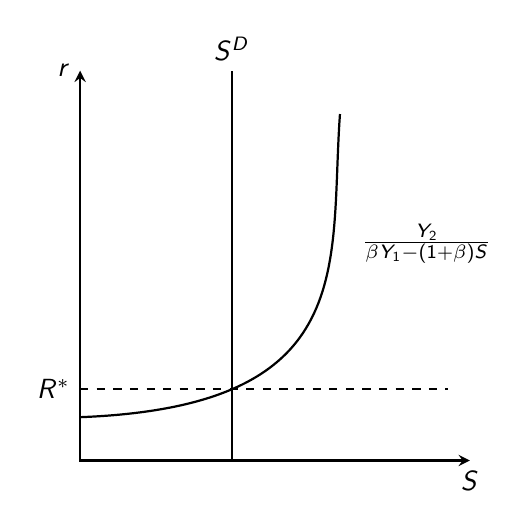
\begin{tikzpicture}[scale=0.55]
						\draw [thick, <->] (0,9) node[left]{\(r\)} -- (0,0) -- (9,0) node[below]{\(S\)};
						\draw [thick] (0,1) .. controls (6.5,1.25) and (5.75,4.5) .. (6,8);
						\draw [thick] (3.5,0) -- (3.5,9) node[above]{\( S^D \)};
						\draw [thick,dashed] (0,1.65) node[left]{\( R^* \)} -- (8.5,1.65);
						\node at (8,5) {\( \frac{Y_2}{\beta Y_1 - (1+\beta) S} \)};
					\end{tikzpicture}
				\end{figure}
			\end{explanationbox}
			\item On two separate figures, show the effect of 
			\begin{enumerate}[(i)]
				\item a decrease in period 1 income \( Y_1 \)
				\item a decrease in period 2 income \( Y_2 \)
			\end{enumerate}
			Provide economic intuition for equilibrium outcomes following the the changes in incomes.
			\begin{explanationbox}
				A decrease in income in period 1 means that the household has less resources available to consume in period 1 than was previously the case. The household wants to transfer resources from period 2 to period 1 in order to help smooth consumption in period 1. In order to do this, the household saves less in period 1 at any given level of the interest rate. Hence, the savings supply curve shifts left. In equilibrium, the decrease in the supply of savings relative to the constant demand for savings leads to an increase in the equilibrium interest rate.
				\begin{figure}[H]
					\centering
					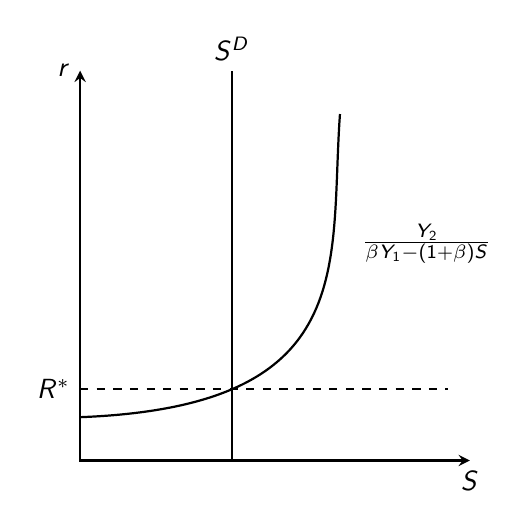
\begin{tikzpicture}[scale=0.55]
						\draw [thick, <->] (0,9) node[left]{\(r\)} -- (0,0) -- (9,0) node[below]{\(S\)};
						\draw [thick] (0,1) .. controls (6.5,1.25) and (5.75,4.5) .. (6,8);
						\draw [thick] (3.5,0) -- (3.5,9) node[above]{\( S^D \)};
						\draw [thick,dashed] (0,1.65) node[left]{\( R^* \)} -- (8.5,1.65);
						\node at (8,5) {\( \frac{Y_2}{\beta Y_1 - (1+\beta) S} \)};
					\end{tikzpicture}
				\end{figure}
				A decrease in income in period 2 means that the household has less resources available to consume in period 2 than was previously the case. The household wants to transfer resources from period 1 to period 2 in order to help smooth consumption in period 2. In order to do this, the household saves more in period 1 at any given level of the interest rate. Hence, the savings supply curve shifts right. In equilibrium, the increase in the supply of savings relative to the constant demand for savings leads to a decrease in the equilibrium interest rate.
			\end{explanationbox}
			\begin{explanationbox}
				\begin{figure}[H]
				\centering
					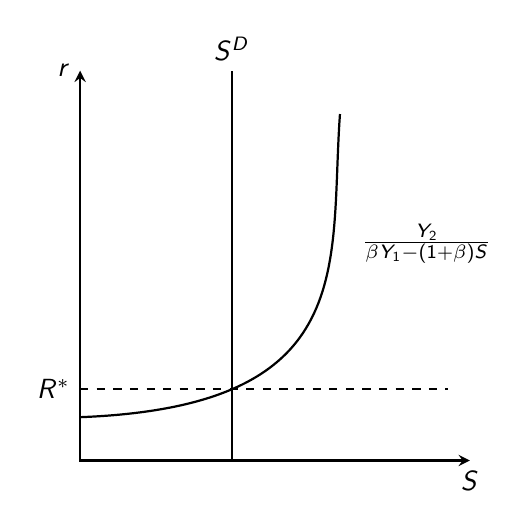
\begin{tikzpicture}[scale=0.55]
						\draw [thick, <->] (0,9) node[left]{\(r\)} -- (0,0) -- (9,0) node[below]{\(S\)};
						\draw [thick] (0,1) .. controls (6.5,1.25) and (5.75,4.5) .. (6,8);
						\draw [thick] (3.5,0) -- (3.5,9) node[above]{\( S^D \)};
						\draw [thick,dashed] (0,1.65) node[left]{\( R^* \)} -- (8.5,1.65);
						\node at (8,5) {\( \frac{Y_2}{\beta Y_1 - (1+\beta) S} \)};
					\end{tikzpicture}
				\end{figure}
			\end{explanationbox}
		\end{enumerate}
	\end{questionbox}
	\begin{questionbox}{Question 2}
		Consider the following two-period household consumption and savings problem. In this problem we will use a power utility function for the household's objective function.
		\begin{align*}
			\max_{C_1,C_2,S} \quad &\frac{C_1^{1-\sigma}}{1 - \sigma} + \beta\frac{C_2^{1-\sigma}}{1-\sigma}\\
			\text{s.t} \quad &C_1 + S = Y_1\\
			&C_2 = Y_2 + SR
		\end{align*}
		where \( R \) is the gross interest rate.
		\begin{enumerate}[(a)]
			\item Write down the inter-temporal budget constraint. With reference to the inter-temporal budget constraint, describe how the interest rate is related to the price of consumption in period 2.
			\begin{explanationbox}
				First rearrange the period 2 budget constraint for savings:
				\[
					S = \frac{C_2}{R}-\frac{Y_2}{R}
				\]
				Substitute this equation into the period 1 budget constraint and rerrange:
				\[
					C_1 + \frac{C_2}{R} = Y_1 + \frac{Y_2}{R}
				\]
				Since this is a budget constraint, the price of consumption in period 1 is equal to 1 (i.e. the numeraire). Then the price of consumption in period 2 is equal to \( \frac{1}{R} \). An \( R \) increase in the interest rate is associated with a decrease in the price of consumption in period 2.
			\end{explanationbox}
			\item Solve for the first order conditions of the problem. Use the first order conditions and the budget constraint(s) to find consumption demands as functions of the interest rate and income.
			\begin{explanationbox}
				First, substitute the inter-temporal budget constraint into the objective function:
				\[
					\max_{C_2} \quad \frac{(C_1+\frac{Y_2}{R}-\frac{C_2}{R})^{1-\sigma}}{1 - \sigma} + \beta\frac{C_2^{1-\sigma}}{1-\sigma}
				\]
				Next, take the first order condition with respect to \( C_2 \):
				\[
					-\frac{1}{R}\left( C_1+\frac{Y_2}{R}-\frac{C_2}{R} \right)^{-\sigma} + \beta C_2^{-\sigma} = 0
				\]
			\end{explanationbox}
			\begin{explanationbox}
				Next, rearrange for \( C_2 \). First, multiply each side of the equation by \( R \) and then raise each side of the equation to the power of \( \frac{-1}{\sigma} \):
				\[
					Y_1 + \frac{Y_2}{R} - \frac{C_2}{R} = (\beta R)^{\frac{-1}{\sigma}} C_2
				\]
				Next, multiply each side of the equation by \( R \) again to help simplify:
				\[
					R Y_1 + Y_2 - C_2 = \beta^{\frac{-1}{\sigma}} R^{1-\frac{1}{\sigma}} C_2
				\]
				Now gather the terms in \( C_2 \), and solve for the period 2 consumption demand:
				\begin{align}
					C_2 = \frac{1}{1 + \beta^{\frac{-1}{\sigma}}R^{1-\frac{1}{\sigma}}} (RY_1 + Y_2) \notag\\
					C_2 = \frac{\beta}{\beta + (\beta R)^{1 - \frac{1}{\sigma}}} (RY_1 + Y_2) \label{3.1}
				\end{align}
				Now solve for consumption demand in period 1 by substituting \cref{3.1} into the inter-temporal budget constraint:
				\begin{align*}
					&C_1 + \frac{\beta}{\beta + (\beta R)^{1 - \frac{-1}{\sigma}}} (RY_1 + Y_2) = Y_1 + \frac{Y_2}{R}\\
					&C_1 = \left( 1 - \frac{\beta}{\beta + (\beta R)^{1 - \frac{1}{\sigma}}} \right) \left( Y_1 +\frac{Y_2}{R} \right)\\
					&C_1 = \left( \frac{(\beta R)^{1 - \frac{1}{\sigma}}}{\beta + (\beta R)^{1 - \frac{1}{\sigma}}} \right) \left( Y_1 +\frac{Y_2}{R} \right)
				\end{align*}
			\end{explanationbox}
			\item Show that when \( \sigma = 1 \), the consumption functions you derived above are identical to those under the log-utility specification discussed in Lecture 3.
			\begin{explanationbox}
				The consumption demand functions in the current problem are:
				\begin{align*}
					C_1 &= \left( \frac{(\beta R)^{1 - \frac{1}{\sigma}}}{\beta + (\beta R)^{1 - \frac{1}{\sigma}}} \right) \left( Y_1 +\frac{Y_2}{R} \right)\\
					C_2 &= \left( \frac{\beta}{\beta + (\beta R)^{1 - \frac{1}{\sigma}}} \right) \left( RY_1 + Y_2 \right)
				\end{align*}
				Set \( \sigma = 1 \), which yields:
				\begin{align*}
					C_1 &= \left( \frac{(\beta R)^0}{\beta + (\beta R)^0} \right) \left( Y_1 +\frac{Y_2}{R} \right)\\
					C_2 &= \left( \frac{\beta}{\beta + (\beta R)^0} \right) \left( RY_1 + Y_2 \right)
				\end{align*}
				Simplifying:
				\begin{align*}
					C_1 &= \left( \frac{1}{\beta + 1} \right) \left( Y_1 + \frac{Y_2}{R} \right)\\
					C_2 &= \frac{\beta R}{\beta + 1} \left( Y_1 + \frac{Y_2}{R} \right)
				\end{align*}
			\end{explanationbox}\pagebreak
			\item Continue to assume that \( \sigma = 1 \). What is the effect of an increase in the interest rate \( R \) on \( C_1 \) and \( C_2 \)?
			\begin{explanationbox}
				In order to show the effect of the interest rate on consumption demands, take the derivative of each function with respect to the interest rate \( R \):
				\begin{align*}
					\frac{\partial C_1}{\partial R} &= -\left( \frac{1}{\beta + 1} \right) \frac{Y_2}{R^2}\\
					\frac{\partial C_2}{\partial R} &= \frac{\beta}{\beta + 1} Y_1
				\end{align*}
				As the interest rate increases, consumption in period 1 declines, while consumption in period 2 increases.\\
				Note that since \( \frac{1}{R} \) is the price of consumption in period 2, an increase in the interest rare effectively reduces the price of \( C_2 \) and increases the price of \( C_1 \).
			\end{explanationbox}
			\item Suppose that income is constant across periods, so \( Y_1 = Y_2 = Y \), and that \( R > 1 \). Now assume that \( \beta = 0 \). Under this parameterization, is \( C_1 \) or \( C_2 \) more sensitive to changes in the interest rate?
			\begin{explanationbox}
				Setting \( Y_1 = Y_2 = Y \) and \( \beta = 0 \), and substituting into the derivatives from above:
				\begin{align*}
					\frac{\partial C_1}{\partial R} &= -\frac{Y}{R^2}\\
					\frac{\partial C_2}{\partial R} &= 0
				\end{align*}
				Under this parameterisation consumption in period 2 is totally insensitive to changes in the interest rate, while consumption in period 1 is still negatively associated with increases in the interest rate.
			\end{explanationbox}
			\item Suppose that income is constant across periods, so \( Y_1 = Y_2 = Y \), and that \( R > 1 \). Now assume that \( \beta = 1 \). Under this parameterisation, is \( C_1 \) or \( C_2 \) more sensitive to changes in the interest rate?
			\begin{explanationbox}
				Setting \( Y_1 = Y_2 = Y \) and \( \beta = 1 \), and substituting into the derivatives from above:
				\begin{align*}
					\frac{\partial C_1}{\partial R} &= -\frac{1}{2}\frac{Y}{R^2}\\
					\frac{\partial C_2}{\partial R} &= \frac{1}{2} Y
				\end{align*}
				Since \( R > 1 \), we have that \( \frac{1}{2}Y \) is greater than \( \frac{1}{2}\frac{Y}{R^2} \). Therefore, \( C_2 \) is more sensitive to changes in the interest rate than is \( C_1 \).
			\end{explanationbox}
		\end{enumerate}
	\end{questionbox}\pagebreak
	\begin{questionbox}{Question 3}
		Consider the following \textbf{three-period} household consumption and savings problem. In this problem, a household lives for three periods. In the final period of life the household retires, earns no income, and must consume any available retirement savings, \( S_3 \). Retirement savings must be put aside in the first period, but nothing can be saved from period 2. In period 1, the household can also put aside savings (or borrow), for period 2, \( S_2 \). In all, the household makes two savings decisions in period 1 - \( S_2,S_3 \) - and one consumption decision in each of the three periods - \( C_1,C_2,C_3 \). The household problem can be described as follows:
		\begin{align*}
			\max_{C_1,C_2,C_3,S_2,S_3} \quad &\log C_1 + \beta\log C_2 + \beta^2\log C_3\\
			\text{s.t} \quad & C_1 + S_2 + S_3 = Y_1\\
			&C_2 = Y_2 + S_2R_2\\
			&C_3 = S_3 R_3
		\end{align*}
		where \( R_2 \) is the interest rate earned on savings in period 2, and \( R_3 \) is the interest rate earning on retirement savings available in period 3.
		\begin{enumerate}[(a)]
			\item Substitute each of the budget constraints into the utility function in order to rewrite the household problem as an \textbf{unconstrained optimisation problem} in the two choice variables \( S_2 \) and S3.
			\begin{explanationbox}
				Substitute the period 1 budget constraint into \( C_1 \); substitute the period 2 budget constraint into \( C_2 \); and substitute the period 3 budget constraint into \( C_3 \). Then the household problem can be written as:
				\[
					\max_{S_2,S_3} \quad \log(Y_1 - S_2 - S_3) + \beta\log(Y_2 - S_2R_2) + \beta^2\log(S_3R_3)
				\]
			\end{explanationbox}
			\item Take the first order conditions for the two savings decisions \( (S_2,S_3) \)
			\begin{explanationbox}
				\begin{align}
					S_2: \quad & \frac{1}{Y_1-S_2-S_3} = \frac{\beta R_2}{Y_2 + S_2R_2} \label{3.2}\\
					S_3: \quad & \frac{1}{Y_1-S_2-S_3} = \frac{\beta^2R_3}{S_3R_3} \label{3.3}
				\end{align}
			\end{explanationbox}
			\item Use the first order conditions to solve for the two savings decisions as functions of incomes and interest rates.
			\begin{explanationbox}
				Rearranging \cref{3.3} for \( S_3 \)
				\begin{equation}
					S_3 = \frac{\beta^2}{1+\beta^2}(Y_1 - S_2) \label{3.4}
				\end{equation}
				Substituting equation \cref{3.4} into \cref{3.2}, and solve for \( S_2 \):
				\begin{align*}
					\frac{1}{Y_1-S_2-S_3} &= \frac{\beta R_2}{Y_2 + S_2R_2}\\
					(Y_2 + S_2R_2) &= \beta R_2 (Y_1 - S_2 - S_3)\\
					(Y_2 + S_2R_2) &= \beta R_2 \left( Y_1 - S_2 - \frac{\beta^2}{1+\beta^2}(Y_1 - S_2) \right)\\
					(Y_2 + S_2R_2) &= \frac{\beta R_2}{1 + \beta^2} Y_1 - \frac{\beta R_2}{1 + \beta^2} S_2\\
					S_2 \left( R_2 + \frac{\beta R_2}{1 + \beta^2} \right) &= \frac{\beta R_2}{1 + \beta^2} Y_1-Y_2\\
					S_2 \left( R_2 + \frac{1 + \beta + \beta^2}{1 + \beta^2} \right) &= \frac{\beta R_2}{1 + \beta^2} Y_1-Y_2\\
					S_2 &= \left( R_2 + \frac{1 + \beta + \beta^2}{1 + \beta^2} \right)^{-1} \left( \frac{\beta R_2}{1 + \beta^2} Y_1-Y_2 \right)
				\end{align*}
			\end{explanationbox}
			\begin{explanationbox}
				Which, tidying up, yields the expression for \( S_2 \):
				\begin{equation}
					S_2 = \frac{\beta}{1 + \beta + \beta^2} Y_1 - \frac{1 + \beta^2}{R_2(1 + \beta + \beta^2)}Y_2 \label{3.5}
				\end{equation}
				Substituting \cref{3.4} into \cref{3.5} to find \( S_3 \):
				\begin{align}
					S_3 &= \frac{\beta^2}{1+\beta^2}(Y_1 - \frac{\beta}{1 + \beta + \beta^2} Y_1 - \frac{1 + \beta^2}{R_2(1 + \beta + \beta^2)}Y_2) \notag \\
					&= \frac{\beta^2}{1+\beta^2}\left( \frac{1 + \beta^2}{R_2(1 + \beta + \beta^2)}Y_1 + \frac{1 + \beta^2}{R_2(1 + \beta + \beta^2)}Y_2 \right) \notag
				\intertext{Which, tidying up, yields the expression for \( S_3 \):}
				S_3 &= \frac{\beta^2}{1 + \beta + \beta^2} \left( Y_1 + \frac{Y_2}{R_2} \right) \label{3.6}
				\end{align}
			\end{explanationbox}
			\item How does the household use the available assets to finance its retirement? How does your answer change when second period income, \( Y_2 \), is very large or very small?
			\begin{explanationbox}
				\begin{itemize}
					\item The household always has positive retirement savings, since \cref{3.6} is always positive. Notice that \( S_2 \) is a function of both period 1 income and period 2 income. But the household can only save for retirement in period 1, when it does not yet have access to period 2 income. This means that the household may borrow against period 2 income, in order to finance retirement savings in period 3. This can be seen from \cref{3.5}. We can see that \( S_2 \) may be negative, if the second term is much larger than the first term. In this case, the household borrows using \( S_2 \) in order to then save in the retirement savings account \( S_3 \).
					\item If \( Y_2 \) is very large, then the second term in \cref{3.5} dominates the first term, and \( S_2 \) is negative. This is the case where the household borrows against period 2 income in order to finance retirement savings.
					\item If \( Y_2 \) is very small, then the second term in \cref{3.5} is smaller than the first term, and \( S_2 \) is positive. In this case, the household is very wealthy in period 1 and does not need to borrow against period 2 income in order to save for retirement. Instead, in period 1 the household saves resources to be consumed in both periods 2 and 3. Thus, when the household is very wealthy in period 1, they will smooth income across both of the subsequent periods by saving through assets \( S_2 \) and \( S_3 \) in period 1.
				\end{itemize}
			\end{explanationbox}
			\item How are retirement savings affected by the second period interest rate \( R_2 \)? How are retirement avings affected by the third period interest rate, \( R_3 \)?
			\begin{explanationbox}
				\begin{itemize}
					\item The effect of \( R_2 \) can be expressed using the derivative of the savings functions with respect to \( R_2 \):
					\begin{align*}
						\frac{\partial S_2}{\partial R_2} &= \frac{1 + \beta^2}{R_2^2 (1 + \beta + \beta^2)}Y_2\\
						\frac{\partial S_3}{\partial R_2} &= \frac{\beta^2}{1 + \beta + \beta^2}\frac{Y_2}{R_2^2}
					\end{align*}
					This shows that an increases in \( R_2 \) results in an increase in \( S_2 \) and a decrease in \( S_3 \). The increase in \( R_2 \) increases the return to savings in period 2, so the household saves more for consumption for period 2 and saves less for retirement in period 3.
				\end{itemize}
			\end{explanationbox}
			\begin{explanationbox}
				\begin{itemize}
					\item The effect of \( R_3 \) can be expressed using the derivative of the savings functions with respect to \( R_3 \):
					\begin{align*}
						\frac{\partial S_2}{\partial R_3} &= 0\\
						\frac{\partial S_3}{\partial R_3} &= 0
					\end{align*}
					In this case, household savings decisions are unaffected by changes in the interest rate during retirement.
				\end{itemize}
			\end{explanationbox}
		\end{enumerate}
	\end{questionbox}
\section{Tutorial 4}
	\begin{questionbox}{Question 1}
		Denote the price of a nominal bond that pays one dollar next period as \( S_t^1 \). Now denote the price of a nominal bond that pays one dollar \textbf{two periods from now} as \( S_t^2 \). Both bonds can be purchased today, but the first pays off next period while the second pays off two periods from now.
		\begin{enumerate}[(a)]
			\item Write down an expression for the nominal rate of return on each bond as a function of the bond price. Rearrange this expression to express the bond prices as functions of the nominal rates of return.
			\begin{explanationbox}
				The nominal return on each bond are:
				\[
					r_t^{n,1} = \frac{1-S_t^1}{S_t^1} \quad r_t^{n,2} = \frac{1-S_t^2}{S_t^2}
				\]
				The bond prices are then expressed as:
				\[
					S_t^1 = \frac{1}{1 + r_t^{n,1}}, \quad S_t^2 = \frac{1}{1 + r_t^{n,2}}
				\]
			\end{explanationbox}
			\item Now write down expressions for the \textbf{real rates of return} on each bond as a function of the bond prices and current and future price levels. Use these expressions to find the \textbf{Fisher Equation} for each of the bonds.
			\begin{explanationbox}
				\begin{itemize}
					\item The real rate of return on the first bond is:
					\begin{align*}
						R_t^1 &= \frac{1/P_{t+1}-S_t^1/P_t}{S_t^1/P_t} = \frac{1}{S_t^1}\frac{P_t}{P_{t+1}} - 1\\
						1 + r_t^1 &= \frac{1}{S_t^1}\frac{P_t}{P_{t+1}}\\
						&= (1+r_t^{n,1}) \frac{1}{1+\pi_{t+1}}
					\end{align*}
					\item The real rate of return on the second bond is:
					\begin{align*}
						R_t^2 &= \frac{1/P_{t+2}-S_t^1/P_t}{S_t^1/P_t} = \frac{1}{S_t^2}\frac{P_t}{P_{t+2}} - 1\\
						1 + r_t^2 &= \frac{1}{S_t^2}\frac{P_t}{P_{t+1}}\frac{P_{t+1}}{P_{t+2}}\\
						&= (1+r_t^{n,2}) \frac{1}{1+\pi_{t+1}} \frac{1}{1+\pi_{t+2}}
					\end{align*}
				\end{itemize}
			\end{explanationbox}
			\begin{explanationbox}
				\begin{itemize}
					\item To find the Fisher equation for the first bond, rewrite with the nominal rate of return on the left hand side, and then expand the expression on the right hand side:
					\begin{align*}
						(1+r_t^{n+1}) &= (1+r_t^1)(1+\pi_{t+1})\\
						&=  1 + r_t^1 + \pi_{t+1} + r_t^1 \pi_{t+1}\\
						&\approx 1 + r_t^1 + \pi_{t+1}
					\end{align*}
					where the final equality follows from the approximation that higher order terms are equal to zero i.e. \( r_t61 \pi_{t+1} \approx 0 \).
					\item To find the Fisher equation for the second bond, follow the same steps as above:
					\begin{align*}
						(1+r_t^{n,2}) &= (1+r_t^2)(1+\pi_{t+1})(1+\pi_{t+2})\\
						&= 1 + r_t^2 + \pi_{t+1} + \pi_{t+2} + r_t^2 \pi_{t+1} + r_t^2 \pi_{t+2} + \pi_{t+1}\pi_{t+2} + r_t^2\pi_{t+1}\pi_{t+2}\\
						&\approx 1 + r_t^2 + \pi_{t+1} \pi_{t+2}
					\end{align*}
				\end{itemize}
			\end{explanationbox}
		\end{enumerate}
	\end{questionbox}
	\begin{questionbox}{Question 2}
		Consider the model from Lecture 4 for household choices over consumption, money holdings, and nominal bonds:
		\begin{align*}
			\max_{C_1,C_2,M,B} \quad &\log C_1 + \omega\log \frac{M}{P_1} + \beta\log C_2 \\
			\text{s.t.} \quad &P_1C_1 + M + B P_1Y_1\\
			&P_2C_2 = P_2Y_2 + M + B (1+r^n)
		\end{align*}
		In class, we showed that the Euler equation is:
		\begin{equation}
			\frac{1}{C_1} = \beta(1+r^n)\frac{P_1}{P_2}\frac{1}{C_2} \label{4.1}
		\end{equation}
		And the money demand equation is given by:
		\begin{equation}
			\frac{M}{P_1} = \omega C_1 \left( \frac{r^n}{1 + r^n} \right)^{-1} \label{4.2}
		\end{equation}
		\begin{enumerate}[(a)]
			\item Rewrite the money demand equation so that the nominal interest rate (i.e. the price) is expressed as a function of money demand (i.e. the quantity). Plot this money demand function on a graph with the interest rate on the y-axis, and money demand on the x-axis.
			\begin{explanationbox}
				The money demand equation is:
					\begin{align*}
						\frac{M}{P_1} &= \omega C_1 \left( \frac{r^n}{1 + r^n} \right)^{-1}\\
						\frac{M}{P_1} r^n &= \omega C_1 (1+r^n)\\
						r^n\left( \frac{M}{P_1} - \omega C_1 \right) &= \omega C_1\\
						r^n &= \frac{\omega C_1}{\left( \frac{M}{P_1} - \omega C_1 \right)}
					\end{align*}
					which, on the final line, is expressed as the interest rate in terms of money demand.
			\end{explanationbox}
			\begin{explanationbox}
				We can plot the money demand function in \( (r^n, M/P_1) \)-space as:
				\begin{figure}[H]
					\centering
					\begin{tikzpicture}[scale=0.55]
						\draw [thick, <->] (0,9) node[left]{\(r^n\)} -- (0,0) -- (9,0) node[below]{\(\frac{M}{P}\)};
						\draw [thick] (1,8) .. controls (1.25,3) and (2.5,1.25) .. (8,1) node [above]{\( M^D \)};
					\end{tikzpicture}
				\end{figure}
			\end{explanationbox}
			\item On a new graph, again plot the money demand curve from the previous question. Now add a money supply curve, such that the quantity of money supplied is constant/inelastic with respect to the interest rate. Be sure to label the equilibrium interest rate. On your graph, show what happen if there is a \textbf{positive money demand shock}, i.e. an increase in the parameter ω. Label the new equilibrium interest rate and quantity of money.
			\begin{explanationbox}
				If the money supply curve is inelastic with respect to the interest rate, it must be vertical in \( (r^n, M/P_1) \)-space.
				\begin{figure}[H]
					\centering
					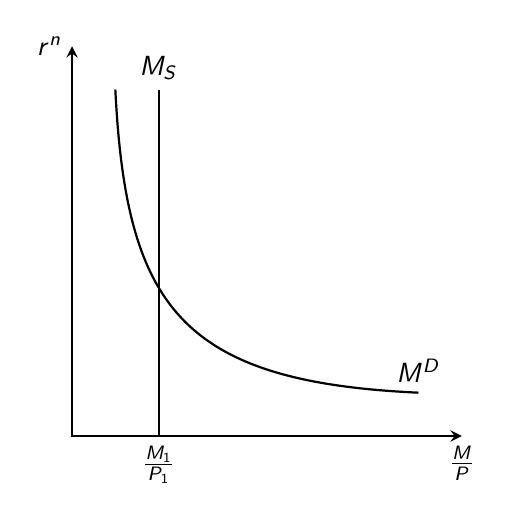
\begin{tikzpicture}[scale=0.55]
						\draw [thick, <->] (0,9) node[left]{\(r^n\)} -- (0,0) -- (9,0) node[below]{\(\frac{M}{P}\)};
						\draw [thick] (1,8) .. controls (1.25,3) and (2.5,1.25) .. (8,1) node [above]{\( M^D \)};
						\draw [thick] (2,0) node [below]{\(\frac{M_1}{P_1}\)} -- (2,8) node [above]{\( M_S \)}; %add r^n
					\end{tikzpicture}
				\end{figure}
				An increase in money demand, \( \omega \), leads to a shift up in the money demand curve. We can see this by taking the derivative of the money demand equation with respect to \( \omega \):
				\[
					\frac{\partial r^n}{\partial \omega} = \frac{C_1}{\left( \frac{M}{P_1} - \omega C_1 \right)} + \frac{\omega C_1^2}{\left( \frac{M}{P_1} - \omega C_1 \right)^2} > 0
				\]
				Since the money supply curve is constant, the increase in the money demand curve leads to an increase in the real interest rate:
			\end{explanationbox}
			\begin{explanationbox}
				\begin{figure}[H]
					\centering
					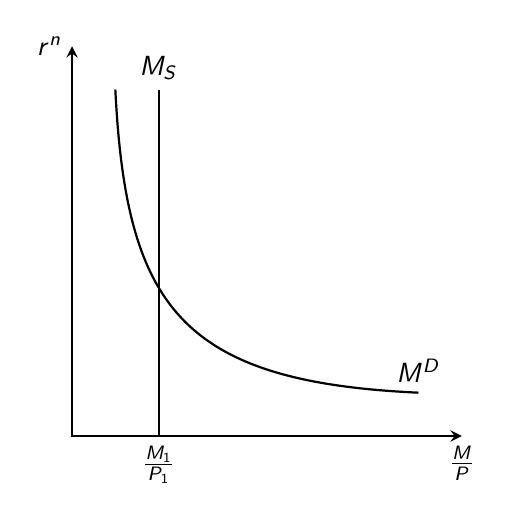
\begin{tikzpicture}[scale=0.55]
						\draw [thick, <->] (0,9) node[left]{\(r^n\)} -- (0,0) -- (9,0) node[below]{\(\frac{M}{P}\)};
						\draw [thick] (1,8) .. controls (1.25,3) and (2.5,1.25) .. (8,1) node [above]{\( M^D \)};
						\draw [thick] (2,0) node [below]{\(\frac{M_1}{P_1}\)} -- (2,8) node [above]{\( M_S \)}; %add r^n and Md'
					\end{tikzpicture}
				\end{figure}
				Since households want to hold more money, but the money supply has not changed, the nominal interest rate on bonds must increase in order to induce households to hold bonds and keep their money holdings at their original quantity.
			\end{explanationbox}
			\item Combine budget constraints and the money demand \cref{4.2} to find an expression for the bond-demand equation as a function of \( C_1 \). As above, rewrite the equation to express the bond demand equation with the interest rate as a function of real bond holdings, \( B/P_1 \). Why is the bond demand curve upward sloping? Use both math and economic intuition in your answer.
			\begin{explanationbox}
				The first period budget constraint after dividing through by \( P_1 \), is:
				\[
					C_1 + \frac{M}{P_1} + \frac{B}{P_1} = Y_1
				\]
				Now substitute in the money demand \cref{4.2}, and rearrange for real bond holdings:
				\begin{align*}
					C_1 + \omega C_1 \left( \frac{r^n}{1+r^n} \right)^{-1} + \frac{B}{P_1} = Y_1\\
					C_1 \left( 1 + \omega \left( 1 + \frac{1}{r^n} \right) \right) + \frac{B}{P_1} = Y_1\\
					\frac{B}{P_1} = Y_1 - C_1 \left( 1 + \omega \left( 1 + \frac{1}{r^n} \right) \right)
				\end{align*}
				Now rearrange the equation so that \( r^n \) is on the left and bond holdings are on the right:
				\[
					r^n = \frac{- \omega C_1}{\frac{B}{P_1} - Y_1 + C_1 (1 + \omega)}
				\]
				Note that \( \frac{B}{P_1} - Y_1 + C_1 (1 + \omega) < 0 \), so the right hand side is positive. Additionally,
				\[
					\frac{\partial r^n}{\partial \frac{B}{P_1}} = \frac{C_1}{\left( \frac{B}{P_1} - Y_1 + C_1 (1 + \omega) \right)^2} > 0
				\]
				so the bond demand curve is upward sloping. Why is this the case? In order to induce households to hold more bonds, the nominal rate of return on those bonds has to increase.
			\end{explanationbox}\pagebreak
			\item Draw the bond demand curve, with \( \frac{B}{P_1} \) on the x-axis, and \( r^n \) on the y-axis. Now suppose a central bank determines how many bonds are available in the bond market. The supply of bonds is constant/inelastic with respect to the interest. Illustrate equilibrium in the bond market, being sure to label the equilibrium interest rate.
			\begin{explanationbox}
				The bond demand curve is upward sloping, while the bond supply curve is vertical:
				\begin{figure}[H]
					\centering
					\begin{tikzpicture}[scale=0.55]
						\draw [thick, <->] (0,9) node[left]{\(r^n\)} -- (0,0) -- (9,0) node[below]{\(\frac{B}{P_1}\)};
						\draw [thick] (1,1) .. controls (1.25,6) and (4,7.75) .. (8,8) node [right]{\( B^D \)};
						\draw [thick] (2.5,0) node [below]{\(\frac{B}{P_1}\)} -- (2.5,8) node [above]{\( B^S \)}; %add r^n
					\end{tikzpicture}
				\end{figure}
			\end{explanationbox}
			\item Suppose the central bank increases the supply of bonds (i.e. by selling bonds into the market). What is the effect on the equilibrium nominal interest rate? Illustrate your answer. What is the effect of this policy on real money holdings? What does this suggest about the central bank’s ability to conduct monetary policy using either the money or bond supply?
			\begin{explanationbox}
				\begin{itemize}
					\item An increase in the supply of bonds results in an increase in the nominal interest rate:
					\item Because the nominal interest rate rises, real money balances held by households decline. This can be seen from the money demand equation.
					\item Because the central bank can manipulate nominal interest rates by \textbf{either} changing the money supply or changing the bond suppl, the ability to conduct monetary policy is una˙ected by the choice of instrument. That is, the central bank can achieve the same monetary goals by either choosing the money supply or by choosing the bond supply.
				\end{itemize}
				\begin{figure}[H]
					\centering
					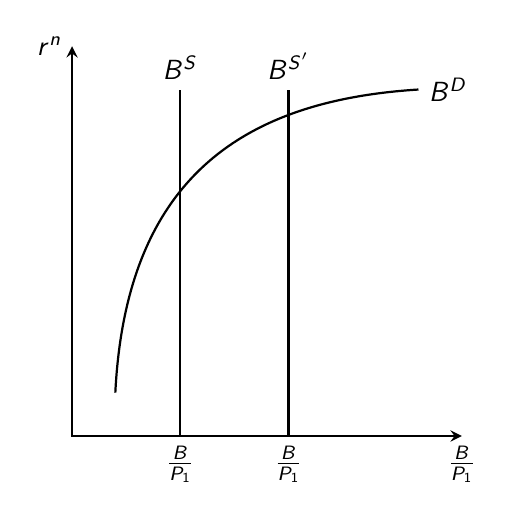
\begin{tikzpicture}[scale=0.55]
						\draw [thick, <->] (0,9) node[left]{\(r^n\)} -- (0,0) -- (9,0) node[below]{\(\frac{B}{P_1}\)};
						\draw [thick] (1,1) .. controls (1.25,6) and (4,7.75) .. (8,8) node [right]{\( B^D \)};
						\draw [thick] (2.5,0) node [below]{\(\frac{B}{P_1}\)} -- (2.5,8) node [above]{\( B^S \)}; %add r^n
						\draw [thick] (5,0) node [below]{\(\frac{B}{P_1}\)} -- (5,8) node [above]{\( B^{S'} \)}; %add r^n'
					\end{tikzpicture}
				\end{figure}
			\end{explanationbox}
		\end{enumerate}
	\end{questionbox}\pagebreak
\section{Tutorial 5}
	\begin{questionbox}{Question 1}
		Consider the following household problem:
		\begin{align*}
			\max_{C_1,C_2,S} \quad &\log C_1 + \beta E[\log C_2]\\
			\text{s.t.} \quad &C_1 + S =\bar{Y}\\
			&C_2 = \bar{Y}_2 + S
		\end{align*}
		where savings earn no interest (i.e. \( r = 0 \)), and the realisation of income in period 2 is \textbf{uncertain}:
		\[
			Y_2 =
			\begin{cases}
				\bar{Y} + x \;\text{with probability}\; \alpha\\
				\bar{Y} - x \;\text{with probability}\; 1 - \alpha
			\end{cases}
		\]
		\begin{enumerate}[(a)]
			\item Write an expression for the expected value of income in period 2. What is the effect on expected income of an increase in the probability \( \alpha \)? Provide an intuitive explanation for why this is the case.
			\begin{explanationbox}
				We can write expected income as:
				\[
					E[Y_2] = \alpha(\bar{Y} + x) + (1 - \alpha)(\bar{Y} - x) = \bar{Y} + 2\alpha x = x
				\]
				The effect of an increase in \( \alpha \) is to increase expected income:
				\[
					\frac{\partial E[Y_2]}{\partial \alpha} = 2x > 0
				\]
				Expected income increases, because an increase in \( \alpha \) shifts the uncertain income towards the positive payoff \( \bar{Y} + x \) and away from the negative payoff \( \bar{Y} - x \). Increasing the probability of a positive payoff leads to an increase in the overall expected payoff.
			\end{explanationbox}
			\item What is the effect on expected income of an increase in the random payoff \( x \)? What is the effect of an increase in \( x \) when: i) \( \alpha = 0.5 \), ii) \( \alpha < 0.5 \). Provide intuitive explanations for your answers.
			\begin{explanationbox}
				Expected income is:
				\[
					E[Y_2] = \bar{Y} + 2\alpha x - x
				\]
				The effect of an increase in the payoff \( x \) is:
				\[
					\frac{\partial E[Y_2]}{\partial x} = 2\alpha - 1
				\]
				\begin{enumerate}[(i)]
					\item When \( \alpha = 0.5 \), the effect of an increase in the payoff \( x \) is:
					\[
						\frac{\partial E[Y_2]}{\partial x} = 2 \times 0.5 - 1 = 0
					\]
					In this case, the two payoffs have equal probabilities, and since the payoffs are symmetric in \( x \) changing x has no effect on the expected value of the payoffs. This is what we call a \textbf{\textcolor{mygreen}{Mean Preserving Spread}} in income.
					\item When \( \alpha < 0.5 \), the effect of an increase in the payoff \( x \) is:
					\[
						\frac{\partial E[Y_2]}{\partial x} < 2 \times 0.5 - 1 = 0
					\]
					That is, the change in expected income is negative. In this case, the probability of the negative payoff \( \bar{Y} - x \) is more likely. So increasing the random component x makes the negative payoff with higher probability worse, which reduces overall expected income.
				\end{enumerate}
			\end{explanationbox}\pagebreak
			\item Substitute the budget constraints into the utility function. Now substitute in the uncertain income \( Y_2 \), and expand the expectations term to show how utility depends on the two possible outcomes for \( Y_2 \). What is the effect on expected utility of an increase in \( \alpha \)? What is the effect on expected utility of an increase in \( x \) (does this depend on the value of \( \alpha \))? Provide intuition for your answers.
			\begin{explanationbox}
				Substituting in the budget constraints we get:
				\[
					U = \log (\bar{Y - S}) + \beta E\left[ \log(\bar{Y}_2 + S) \right]
				\]
				Expanding the expected value term using the definition of period 2 income:
				\[
					U = \log (\bar{Y}- S) + \beta[\alpha\log(\bar{Y} + x + S) + 1-\alpha \log(\bar{Y} - x + S)]
				\]
				The effect on utility of an increase in \( \alpha \) is:
				\[
					\frac{\partial U}{\partial \alpha} = \beta\left[ \log(\bar{Y} + x + S) - \log(\bar{Y} - x + S) \right] > 0
				\]
				Note that \( \log(\bar{Y} + x + S) > \log(\bar{Y} - x + S) \). So an increase in \( \alpha \) increases utility. Again, an increase in \( \alpha \) shifts uncertain income towards the the positive payoff \( \bar{Y} + x \) and away from the negative payoff \( \bar{Y} - x \). Increasing the probability of a positive payoff leads to an increase in the overall expected payoff, which increases utility over outcomes in period 2. The effect no utility of an increase in \( x \) is:
				\[
					\frac{\partial U}{\partial x} = \beta \left[ \alpha\frac{1}{\bar{Y} + x + S} - (1-\alpha)\frac{1}{\bar{Y} - x + S} \right] < 0 \;\text{for sufficiently small}\; \alpha
				\]
				Since \( \bar{Y} + x + S \), we know that \( \frac{1}{\bar{Y} + x + S} < \frac{1}{\bar{Y} - x + S} \). As long as \( \alpha \) is sufficiently small (low probability of good payoff), \( \alpha\frac{1}{\bar{Y} + x + S} < (1-\alpha)\frac{1}{\bar{Y} - x + S} \). In that case, an increase in \( x \) \textbf{decreases} utility. With small \( \alpha \), the bad payoff− is more likely, so an increase in the losses experienced under the bad payoff makes outcomes in period 2 worse, which reduces expected utility.
			\end{explanationbox}
			\item Derive the Consumption Euler Equation for the household's problem. Write the Euler Equation as a function of the two possible outcomes for consumption in period 2: \( C_2^+ = \bar{Y} + x + S \) and \( C_2^- = \bar{Y} - x + S \).
			\begin{explanationbox}
				From the answer to Part c), the household’s problem is:
				\[
					\max_S \log (\bar{Y}- S) + \beta \left[ \alpha\log(\bar{Y} + x + S) + 1-\alpha \log(\bar{Y} - x + S) \right]
				\]
				Taking the first order condition with respect to S:
				\[
					\frac{1}{\bar{Y}-S} = \beta\left[ \log(\bar{Y} + x + S) - \log(\bar{Y} - x + S) \right]
				\]
				Substituting in the consumption terms for the budget constraints, we get the Euler equation:
				\[
					\frac{1}{C_1} = \beta \left[ \alpha\frac{1}{C+2^+} + (1-\alpha) \frac{1}{C_2^-} \right]
				\]
				where the Marginal Utility of Consumption in period 1 is: \( \frac{1}{C_1} \). And the Marginal Utility of Consumption in period 2 is: \( \beta \left[ \alpha\frac{1}{C+2^+} + (1-\alpha) \frac{1}{C_2^-} \right] \)
			\end{explanationbox}\pagebreak
			\item Recall from class that one side of the Euler Equation represents the Marginal Utility of Consumption in period 1, while the other side of the equation represents the (Expected) Marginal Utility of Consumption in period 2. What is the effect on the expected marginal utility of consumption in period 2 of an increase in \( \alpha \)? What do you expect this increase in \( \alpha \) to have on consumption in period 1? What about savings? Note: You do not need to explicitly solve for consumption functions to answer this question. Instead, use the Euler equation to justify your answer.
			\begin{explanationbox}
				\begin{itemize}
					\item The Euler equation was:
					\[
						\frac{1}{C_1} = \beta \left[ \alpha\frac{1}{C+2^+} + (1-\alpha) \frac{1}{C_2^-} \right]
					\]
					\item The effect of an increase in \( \alpha \) on period 2 marginal utility is:
					\[
						\frac{\partial MU_2}{\partial \alpha} = \beta \left[ \frac{1}{\bar{Y} + x + S} - \frac{1}{\bar{Y} - x + S} \right] < 0
					\]
					\item Increasing the probability of the good payoff in period 2 leads to a decrease in marginal utility in period 2.
					\item A decrease in marginal utility in period 2 must be matched by a decrease in marginal utility in period 1, via the Euler Equation. Therefore, \( C_1 \) must \textbf{increase}. This also implies that savings in period 1 must \textbf{decrease}. So an increase in uncertainty that shifts probability towards good payoffs in period 2 results in more consumption in period 1 and less savings.
				\end{itemize}
			\end{explanationbox}
			\item Again referring to the Consumption Euler Equation. What is the effect on the expected marginal utility of consumption in period 2 of an increase in x? What do you expect this increase in \( x \) to have on consumption in period 1? What about savings? Note: You do not need to explicitly solve for consumption functions to answer this question. Instead, use the Euler equation to justify your answer. You may also assume that \( \alpha \) is close to zero.
			\begin{explanationbox}
				\begin{itemize}
					\item The Euler equation was:
					\[
						\frac{1}{C_1} = \beta \left[ \alpha\frac{1}{C+2^+} + (1-\alpha) \frac{1}{C_2^-} \right]
					\]
					\item The effect of an increase in \( x \) on period 2 marginal utility is:
					\[
						\frac{\partial MU_2}{\partial x} = \beta \left[ -\alpha\frac{1}{\left( \bar{Y} + x + S \right)^2} - \frac{1}{\left( \bar{Y} - x + S \right)^2} \right] > 0 \; \text{for sufficiently small } \alpha
					\]
					\item So an increase in x increases marginal utility of consumption in period 2.
					\item An increase in marginal utility in period 2 must be matched by an increase in marginal utility in period 1, via the Euler Equation. Therefore, \( C_1 \) must \textbf{decrease}. This also implies that savings in period 1 must \textbf{increase}. So a decrease in the payoff in a bad state that is more likely (i.e. low \( \alpha \)) results in less consumption in period 1 and more savings.
				\end{itemize}
			\end{explanationbox}
		\end{enumerate}
	\end{questionbox}
	\begin{questionbox}{Question 2}
		Consider the following household problem:
		\begin{align*}
			\max_{C_1,C_2,B} \quad &\log C_1 + \beta E[\log C_2]\\
			\text{s.t} \quad &C_1 + \beta = Y_1\\
			&C_2 = Y_2 + \bar{R}B
		\end{align*}
		where the \( B \) has an uncertain payoff \( \bar{R} \):
		\[
			\bar{R}=
			\begin{cases}
				R \;\text{with probability}\; \alpha\\
				0 \;\text{with probability}\; 1 - \alpha
			\end{cases}
		\]
		In the good state of the world, the bond pays off with interest \( R \). In the bad state of the world, the bond pays out nothing: the household loses both the interest payment and the initial investment in the bond. You can think of this as a situation where bonds may suffer from \textbf{default risk}, where borrowers are unable to repay the bond in bad states of the world.
			\begin{enumerate}[(a)]
				\item Substitute the budget constraints into the utility function. Now substitute in the uncertain bond payoff \( \bar{R} \), and expand the expectations term to show how utility depends on the two possible outcomes for the interest rate \( \bar{R} \). What is the effect on expected utility of an increase in \( \alpha \)?
				\begin{explanationbox}
					Substituting in the budget constraints we get:
					\[
						U = \log (Y_1 - B) + \beta E\left[ \log Y_2 + \bar{R} B \right]
					\]
					Expanding the expected value term using the definition of period 2 income:
					\[
						U = \log (Y_1 - B) + \beta \left[ \alpha \log (Y_2 + RB) + (1-\alpha)\log (Y_2) \right]
					\]
					An increase in \( \alpha \) yields:
					\[
						\frac{\partial U}{\partial \alpha} = \beta [\log (Y_2 + RB) - \log(Y_2)] > 0
					\]
					That is, utility is increasing as the probability of the good payoff in the bond increases.
				\end{explanationbox}
				\item Solve for the household’s bond equation. What is the effect on household bond holdings of an increase in \( \alpha \)? What is the effect on bond holdings of an increase in the interest rate in the good state, \( R \)? Provide economic intuition for your answers.
				\begin{explanationbox}
					To solve for the bond equation, take the household problem after having substituted in the budget constraints:
					\[
						\max_B \log (Y_1 - B) + \beta \left[ \alpha \log (Y_2 + RB) + (1-\alpha)\log (Y_2) \right]
					\]
					Now take the first order condition with respect to bonds:
					\begin{align*}
						\frac{1}{Y_1 - B} &= \beta\alpha \frac{R}{Y_2 + RB}\\
						Y_2 + RB &= \beta\alpha R (Y_1 - B)\\
						RB + \beta\alpha RB &= \beta\alpha RY_1-Y_2\\
						BR(1+\beta\alpha) &= \beta\alpha RY_1-Y_2\\
						B &= \frac{\beta\alpha RY_1-Y_2}{R(1+\beta\alpha)}\\
						B &= \frac{\beta\alpha Y_1}{(1+\beta\alpha)}-\frac{Y_2}{R(1+\beta\alpha)}
					\end{align*}
					The effect on bond holdings of an increase in \( \alpha \) is:
					\begin{align*}
						\frac{\partial B}{\partial \alpha} &= \frac{\beta}{\beta\alpha + 1} Y_1 - \beta\frac{\beta\alpha}{(\beta\alpha + 1)^2}Y_1 + \beta R \frac{1}{(R(\beta\alpha +1))^2}Y_2\\
						&= \frac{\beta(\beta\alpha+1)}{(\beta\alpha+1)^2}Y_1 - \beta\frac{\beta\alpha}{(\beta\alpha+1)^2}Y_1 + \beta R \frac{1}{(R(\beta\alpha+1))^2}Y_2\\
						&= \frac{\beta^2\alpha+\beta}{(\beta\alpha+1)^2}Y_1 - \frac{\beta^2\alpha}{(\beta\alpha+1)^2}Y_1 + \frac{\beta R}{(R(\beta\alpha+1))^2}Y_2\\
						&= \frac{\beta^2\alpha+\beta-\beta^2\alpha}{(\beta\alpha+1)^2}Y_1 + \frac{\beta R}{(R(\beta\alpha+1))^2}Y_2\\
						&= \frac{\beta}{(\beta\alpha+1)^2}Y_1 + \frac{\beta R}{(R(\beta\alpha + 1))^2}Y_2\\
						&> 0
					\end{align*}
				\end{explanationbox}
				\begin{explanationbox}
					Increasing the probability the payoff in the good state increases the expected value of the bond, which increases household demand to hold the bond. Thus, an increase in \( \alpha \) increases \( B \).
					The effect on bond holdings of an increase in \( R \) is:
					\[
						\frac{\partial B}{\partial R} = \frac{Y_2(1+\beta\alpha)}{(R(1+\beta\alpha))^2} > 0
					\]
					Increasing the interest payoff in the good state increases the expected value of the bond, which increases household demand to hold the bond. Thus, an increase in \( R \) increases \( B \).
				\end{explanationbox}
				\item Consider households that have more or less income in period 1 (i.e high \( Y_1 \) vs. low \( Y_1 \)). Which of these households are more sensitive to changes in the probability of a good payoff (i.e. an increase in \( \alpha \))? Provide some economic intuition for your answer.
				\begin{explanationbox}
					Consider again the effect on bond holdings of an increase in \( \alpha \) is:
					\[
						\frac{\partial B}{\partial \alpha} = \frac{\beta}{(\beta\alpha+1)^2}Y_1 + \frac{\beta R}{(R(\beta\alpha + 1))^2}Y_2
					\]
					Notice that the higher is \( Y_1 \), the larger is \( \frac{\partial B}{\partial \alpha} \) We can also see this by taking the second derivative with respect to \( Y_1 \):
					\[
						\frac{\partial^2 B}{\partial \alpha \partial Y_1} = \frac{\beta}{(1+\alpha\beta)^2} > 0
					\]
					That is: the sensitivity to changes in \( \alpha \) is increasing in period 1 income.\\
					The intuition for this result is that households with greater income in period 1 have more resources with which take gambles on the risky payoff provided by the bond. As the probability of the good state increases, high income households can afford to reallocate even more resources toward the risky bond.
				\end{explanationbox}
				\item Consider an extreme case where the interest rate on the bond goes to infinity \( R \rightarrow \infty \) but the probability of the good state goes to zero \( \alpha \rightarrow 0 \). What is the household’s desired bond holdings in this case? Provide economic intuition for your answer.
				\begin{explanationbox}
					Household bond holdings in this case are:
					\begin{align*}
						\underset{R \rightarrow \infty,\alpha \rightarrow 0}{B} &= \frac{1}{1+0\beta} \left( \beta \times 0 \times Y_1 - \frac{Y_2}{\infty} \right) \\
						&= 0
					\end{align*}
					Although the return on the bond is extremely high, there is zero probability that this payoff ever occurs. Note, though, that the household also does not want to borrow using the bond. This is because the hosuehold does not want to repay a bond with infinite interest in the state that will surely occur (since \( \alpha = 0, 1 - \alpha = 1 \)).
				\end{explanationbox}
			\end{enumerate}
	\end{questionbox}
\section{Tutorial 6}
	\begin{questionbox}{Question 1}
		Consider the simple present discounted value formula for an asset:
		\begin{equation}
			P_t = E_t \left( \frac{P_{t+1} + D_{t+1}}{R} \right) \label{6.1}
		\end{equation}
		where \( P_t \) is the price of the asset, \( P_{t+1} \) is the resale price of the asset next period, \( D_{t+1} \) is a dividend paid by the asset next period, and \( R \) is the interest rate used for discounting future values.
		\begin{enumerate}[(a)]
			\item Take \Cref{6.1} and iterate forward one period to show next period's price as a function of the following period's price and dividend. Next, substitute this pricing equation back into (\ref{6.1}) to express the current period asset price as a function of period \( t+1 \) and \( t+2 \) prices and dividend payments.
			\begin{explanationbox}
				Iterating forward one period:
				\[
					P_{t+1} = E_{t+1} \left( \frac{P_{t+2} + D_{t+2}}{R} \right)
				\]
				Substituting into (\ref{6.1}),
				\begin{align*}
					P_t &= E_t \left( \frac{E_{t+1} \left( \frac{P_{t+2} + D_{t+2}}{R} \right) + D_{t+1}}{R} \right)\\
					&=E_t \left( \frac{P_{t+2} + D_{t+2}}{R^2} + \frac{D_{t+1}}{R} \right)
				\end{align*}
				where the second line follows from the Law of Iterated Expectations, i.e.: \( E_t[R_{t+1}(x_{t+1})] = E_t(x_{t+1}) \). Note that our new pricing equation is a function of prices two periods ahead, \( P_{t+2} \) and two periods of dividends \( D_{t+1},D_{t+2} \).
			\end{explanationbox}
		\end{enumerate}
		Now we will construct presented discounted pricing formulas for assets with different rules for future dividends and prices.
		\begin{enumerate}[resume*]
			\item Consider an asset that can be bought today at price \( P_t \). The asset pays a dividend in the following two periods \( (D_{t+1},D_{t+2}) \). The asset can be resold next period \( (t+1) \), but it cannot be resold in the following period \( (t+2) \). First, write down the pricing formula at time \( t \). Next, write down the pricing formula at time \( t+1 \). Finally, substitute the pricing formula at time \( t+1 \) into the pricing formula at time \( t \) to express the price \( P_t \) as a function of period \( t+1 \) and \( t+2 \) prices and dividends. How does this asset price differ from the formula you derived in part (a)?
			\begin{explanationbox}
				The period \( t \) price is:
				\[
					P_t = E_t \left( \frac{P_{t+1} + D_{t+1}}{R} \right)
				\]
				The period \( t+1 \) price is:
				\[
					P_{t+1} = E_{t+1}\left( \frac{D_{t+2}}{R} \right)
				\]
				Since the asset cannot be resold at \( t+2 \) the price at \( t+1 \) is a function of the dividend only. Substituting back into the period t pricing formlua:
				\begin{align*}
					P_t &= E_t \left( \frac{E_{t+1} \left( \frac{D_{t+2}}{R} \right) + D_{t+1}}{R} \right)\\
					&=E_t \left( \frac{D_{t+2}}{R^2} + \frac{D_{t+1}}{R} \right)
				\end{align*}
				where the second line, again, follows from the law of iterated expectations.
			\end{explanationbox}
			\begin{explanationbox}
				This asset price contains the discounted value of dividends in periods \( t+1 \) and \( t+2 \), as in the asset pricing formula in part (a). However, the price is not a function of the period \( t+2 \) price, sine this asset cannot be resold in period \( t+1 \). Thus, the value of this asset is only a function of is dividend payments, not its future resale value.
			\end{explanationbox}
			\item Consider an asset that can be bought today at price \( P_t \). The asset pays a dividend next period \( (D_{t+1}) \), but pays no dividend in the following period. The asset can be resold in both periods \( t+1 \) and \( t+2 \). First, write down the pricing formula at time \( t \). Next, write down the pricing formula at time \( t+1 \). Finally, substitute the pricing formula at time \( t+1 \) into the pricing formula at time \( t \) to express the price \( P_t \) as a function of period \( t+1 \) and \( t+2 \) prices and dividends. How does this asset price differ from the formula you derived in part (a)?
			\begin{explanationbox}
				The period \( t \) price is:
				\[
					P_t = E_t \left( \frac{P_{t+1} + D_{t+1}}{R} \right)
				\]
				The period \( t+1 \) price is:
				\[
					P_{t+1} = E_{t+1}\left( \frac{P_{t+2}}{R} \right)
				\]
				Since the asset can be resold at \( t+2 \) but pays no dividend in this period, the price at \( t+1 \) is a function of the future price only.\\
				Substituting back into the period t pricing formlua:
				\begin{align*}
					P_t &= E_t \left( \frac{E_{t+1} \left( \frac{P_{t+2}}{R} \right) + D_{t+1}}{R} \right)\\
					&=E_t \left( \frac{P_{t+2}}{R^2} + \frac{D_{t+1}}{R} \right)
				\end{align*}
				where the second line, again, follows from the law of iterated expectations.\\
				This asset price contains the discounted value of the price at period \( t+2 \), as in the asset pricing formula in part (a). However, the price is only a function of the period \( t+1 \) dividend, since this asset does not pay a dividend in period \( t+2 \).
			\end{explanationbox}
			\item Consider an asset that can be bought today at price \( P_t \). The asset pays no dividend next period, but does pays a dividend in the following period \( D_{t+2} \), but does pays a dividend in the following period. The asset can be resold in the next period \( t+1 \) but cannot be resold at period \( t+2 \). First, write down the pricing formula at time \( t \). Next, write down the pricing formula at time \( t+1 \). Finally, substitute the pricing formula at time \( t+1 \) into the pricing formula at time \( t \) to express the price \( P_t \) as a function of period \( t+1 \) and \( t+2 \) prices and dividends. How does this asset price differ from the formula you derived in part (a)?
			\begin{explanationbox}
				The period \( t \) price is:
				\[
					P_t = E_t \left( \frac{P_{t+1}}{R} \right)
				\]
				The period \( t+1 \) price is:
				\[
					P_{t+1} = E_{t+1}\left( \frac{D_{t+2}}{R} \right)
				\]
				Since the asset can be resold at \( t+2 \) but pays no dividend in this period, the price at \( t+1 \) is a function of the future price only.\\
				Substituting back into the period \( t \) pricing formlua:
				\begin{align*}
					P_t &= E_t \left( \frac{E_{t+1} \left( \frac{D_{t+2}}{R} \right)}{R} \right)\\
					&=E_t \left( \frac{D_{t+1}}{R^2} \right)
				\end{align*}
				This asset price contains the discounted value of the dividend at period \( t+2 \), as in the asset pricing formula in part (a). However, the price is not a function of either a period \( t+1 \) dividend or a period \( t+2 \) asset price, since this asset does not pay a dividend in period \( t+1 \) and cannot be resold in period \( t+2 \).
			\end{explanationbox}
		\end{enumerate}
	\end{questionbox}
	\begin{questionbox}{Question 2}
		Again, consider the simple present discounted value formula for an asset:
		\begin{equation}
			P_t = E_t \left( \frac{P_{t+1} + D_{t+1}}{R} \right) \label{6.2}
		\end{equation}
		where \( P_t \) is the price of the asset, \( P_{t+1} \) is the resale price of the asset next period, \( D_{t+1} \) is a dividend paid by the asset next period, and \( R \) is the interest rate used for discounting future values.
		\begin{enumerate}[(a)]
			\item Suppose this asset is held for 3 periods and then resold, now show how \cref*{6.2} can be expressed as a function of future dividends and prices.
			\begin{explanationbox}
				The asset pricing formulas at periods \( t,t+1 \) and \( t+2 \) are:
				\begin{align*}
					P_t &= E_t \left( \frac{P_{t+1} + D_{t+1}}{R} \right)\\
					P_{t+1} &= E_{t+1} \left( \frac{P_{t+2} + D_{t+2}}{R} \right)\\
					P_{t+2} &= E_{t+2} \left( \frac{P_{t+3} + D_{t+3}}{R} \right)
				\end{align*}
				Substituting these into the period \( t \) pricing formlua, we have:
				\begin{align*}
					P_t &= E_t \left( \frac{E_{t+1} \left( \frac{E_{t+2} \left( \frac{P_{t+3} + D_{t+3}}{R} \right) + D_{t+2}}{R} \right) + D_{t+1}}{R} \right)\\
					&= E_t \left( \frac{P_{t+3} + D_{t+3}}{R^3} + \frac{D_{t+2}}{R^2} + \frac{D_{t+1}}{R} \right)
				\end{align*}
				where we used the Law of Iterated Expectations for the second step.
			\end{explanationbox}
			\item Suppose this asset is held for 5 periods and then resold, now show how \cref{6.2} can be expressed as a function of future dividends and prices.
			\begin{explanationbox}
				The asset pricing formulas at periods \( t,t+1,t+2,t+3,t+4 \) and \( t+5 \) are:
				\begin{align*}
					P_t &= E_t \left( \frac{P_{t+1} + D_{t+1}}{R} \right)\\
					P_{t+1} &= E_{t+1} \left( \frac{P_{t+2} + D_{t+2}}{R} \right)\\
					P_{t+2} &= E_{t+2} \left( \frac{P_{t+3} + D_{t+3}}{R} \right)\\
					P_{t+3} &= E_{t+3} \left( \frac{P_{t+4} + D_{t+4}}{R} \right)\\
					P_{t+4} &= E_{t+4} \left( \frac{P_{t+5} + D_{t+5}}{R} \right)
				\end{align*}
			\end{explanationbox}
			\begin{explanationbox}
				Substituting these into the period \( t \) pricing formlua, we have:
				\begin{align*}
					P_t &= E_t \left( \frac{E_{t+1} \left( \frac{E_{t+2} \left( \frac{E_{t+3} \left( \frac{E_{t+4} \left( \frac{P_{t+5} + D_{t+5}}{R} \right) + D_{t+4}}{R} \right) + D_{t+3}}{R} \right) + D_{t+2}}{R} \right) + D_{t+1}}{R} \right)\\
					&= E_t \left( \frac{P_{t+5} + D_{t+5}}{R^5} + \frac{D_{t+4}}{R^4}+ \frac{D_{t+3}}{R^3}+ \frac{D_{t+2}}{R^2} + \frac{D_{t+1}}{R} \right)
				\end{align*}
				where we used the Law of Iterated Expectations for the second step.
			\end{explanationbox}
			\item Suppose this asset is held for an arbitrary large \( K \) periods and then resold, now show how \cref{6.2} can be expressed as a function of future dividends and prices. Suppose \( K \) tends to infinity. What is the no bubble condition for this asset? Write down the infinite-horizon present discount value formula after imposing the no bubble condition.
			\begin{explanationbox}
				We can now generalise from our previous calculations. We can see that for any future period \( t+K \), the asset pricing formula must have all of the discounted dividend flows from \( t+1 \) up until \( t+K \), and it has the \( t+K \) discounted price. This suggests that a generic \( K \)-period horizon yields the pricing formula:
				\[
					P_t = E_t \left( \frac{P_{t+K} + D_{t+K}}{R^K} + \dots + \frac{D_{t+2}}{R^2} + \frac{D_{t+1}}{R} \right)
				\]
				We can then simplify this expression by summing up over all of the dividend terms and allowing for appropriate discounting, and keeping the final pricing term:
				\[
					P_t = E_t \sum_{k=1}^\infty \left( \frac{D_{t+k}}{R^k} \right) + E_t \left( \frac{P_{t+K}}{R^K} \right)
				\]
				As \( K\rightarrow\infty \), the No Bubble Condition states that the discounted far-future resale price of the asset must shrink to zero:
				\[
					\lim_{k\rightarrow\infty} E_t \left( \frac{P_{t+K}}{R^K} \right)
				\]
				And this yields the present discounted formula:
				\[
					P_t = E_t \sum_{k=1}^\infty \left( \frac{D_{t+k}}{R^k} \right)
				\]
			\end{explanationbox}
			\item Consider the asset represented by oil futures contracts traded in the midst of the COVID pandemic in 2020. These assets are purchased at a price \( P_t \), they payoff a dividend Dt+1 next period reflecting the value of the oil delivered next period, but the contracts can also be resold next period at price \( P_{t+1} \). The one difference from the assets we have considered so far is that delivery of the oil next period requires the investor to pay to store the oil at cost \( C_{t+1} \). Write down the infinite horizon asset pricing formula for this asset. Can the price of this asset ever be negative? If so, under what conditions would this occur?
			\begin{explanationbox}
				\begin{itemize}
					\item The asset pricing formula for the described oil contract can be written as:
					\[
						P_t = E_t \sum_{k=1}^\infty \left( \frac{D_{t+k} - C_{t+k}}{R^k} \right) = E_t \sum_{k=1}^\infty \left( \frac{D_{t+k}}{R^k} \right) - E_t \sum_{k=1}^\infty \left( \frac{C_{t+k}}{R^k} \right)
					\]
					\item The asset price depends on the presented discounted stream of dividends and the present discounted stream of holding costs.
					\item This asset may have a negative price if the present discounted holding costs are larger than the present discounted stream of dividend payments. During the COVID pandemic, oil holding costs rose because little oil was being consumed and all storage facilities were near capacity, while the value of oil (the dividend) fell due to lack of demand.
				\end{itemize}
			\end{explanationbox}
			\item Consider an asset that pays no dividends, e.g. Apple Inc in its recent history. This asset is purchased at a price \( P_t \), pays no dividend in any period, but can be resold next period at price \( P_{t+1} \). Show how the price of this asset can be expressed as a function of future prices. Can the asset price be positive if the No Bubble Condition is satisfied? If the asset pays no dividend, where does the value of the asset come from?
			\begin{explanationbox}
				\begin{itemize}
					\item From our previous answers, we can simply plug in a dividend of zero and express the current asset price as:
					\[
						P_t = E_t \left( \frac{P_{t+K}}{R^K} \right)
					\]
					\item So the asset price is simply a function of the presented discounted future price.
					\item If the No Bubble Condition was satisfied, this asset would have zero price. So the asset cannot have a positive valuation if it pays no dividend and the No Bubble Condition is satisfied.
					\item The value of asset is derived entirely from its future resale value. Essentially, the value of the asset is entirely due to the ``bubble'' term: the expectation that the asset will continue to be valued in the future.
				\end{itemize}
			\end{explanationbox}
		\end{enumerate}
	\end{questionbox}
\section{Tutorial 8}
	\begin{questionbox}{Question 1}
		Consider a two-period model of the housing market. There are three agents in the housing market: Renters, Homeowners, and Investors.\\
		The problem of a renter:
		\begin{align*}
			\max_{c_1^r,C_2^r,H^r,B^r}\quad &\alpha\log C_1^r + (1-\alpha)\log H^r + \beta\alpha C_2^r\\
			\text{s.t.}\quad &C_1^r + \rho H^r = Y_1^r + B^r\\
			&C_2^r + RB^r = Y_2^r
		\end{align*}
		where the super-script \( r \) denotes renter variables. \( H^r \) is the size of rental property chosen, \( \rho \) is the rental rate paid by the renter, and the renter borrows \( B^r \) and repays interest \( R \) on this borrowing.\\
		The problem of a homeowner:
		\begin{align*}
			\max_{c_1^o,C_2^o,H^o,B^o}\quad &\alpha\log C_1^o + (1-\alpha)\log H^o + \beta\alpha C_2^o\\
			\text{s.t.}\quad &C_1^o + P_1 H^o = Y_1^o + B^o\\
			&C_2^o + R^oB^o = Y_2^o + (1-\delta)P_2H^o
		\end{align*}
		where the super-script \( o \) denotes homeowner variables. \( H^o \) is the size of a house owned by a homeowner, \( P_1,P_2 \) are the prices of houses in period 1 and 2, \( \delta \) is the rate of depreciation on housing, and the homeowner borrows \( B^o \) and repays interest \( R^o \) on this borrowing.\\
		The problem of a investor:
		\begin{align*}
			\max_{c_1^i,C_2^i,H^i,B^i}\quad &\log C_1^i + \beta C_2^i\\
			\text{s.t.}\quad &C_1^i + P_1 H^i = Y_1^i + B^i + \rho H^i\\
			&C_2^i + R^iB^i = Y_2^i + (1-\delta-\tau)P_2H^i\\
			&H^i \geq 0
		\end{align*}
		where the super-script \( i \) denotes investor variables. The investor borrows \( B^i \) and repays interest \( R^i \) on this borrowing. Unlike homeowners, investors must pay a \( \tau \) on the sale of property by investors.
		\begin{enumerate}[(a)]
			\item Solve for the first order conditions of the renting household. Use the first order conditions to illustrate the renter's rental optimality condition and Euler equation.
			\begin{explanationbox}
				The Lagrangian function for the rental household is:
				\[
					\mathcal{L} = \alpha\log C_1^r + (1-\alpha)\log H^r + \beta\alpha C_2^r + \lambda_1(Y_1^r + B^r - C_1^r - \rho H^r) + \lambda_2(Y_2^r - C_2^r - RB^r)
				\]
				The first order conditions are:
				\begin{align}
					C_1^r:\quad &\alpha\frac{1}{C_1^r} = \lambda_1 \label{8.1}\\ 
					C_2^r:\quad &\beta\alpha\frac{1}{C_2^r} = \lambda_2 \label{8.2}\\ 
					H^r:\quad &(1-\alpha)\frac{1}{H^r} = \lambda_1\rho \label{8.3}\\ 
					B^r:\quad &\lambda_1 = \lambda_2 R \label{8.4}
				\end{align}
				Using (\ref{8.1}), (\ref{8.2}) and (\ref{8.4}) to get the Euler equation:
				\[
					\frac{1}{C_1^r} = \beta R \frac{1}{C_2^r}
				\]
				Using (\ref{8.1}) and (\ref{8.3}) to get the rental choice optimality condition:
				\[
					\frac{(1-\alpha)}{\alpha} \frac{1/H^r}{1/C^r_1} = \rho
				\]
			\end{explanationbox}
			\item Solve for the first order conditions of the homeowner household. Use the first order conditions to illustrate the homeowner's Euler equations for bonds and housing. Use the two Euler equations to find a housing asset price equation for the homeowner.
			\begin{explanationbox}
				The Lagrangian function for the homeowner household is:
				\begin{align*}
					\mathcal{L} &= \alpha\log C_1^o + (1-\alpha)\log H^o + \beta\alpha C_2^o + \lambda_1(Y_1^o + B^o - C_1^o - P_1 H^o)\\
					&+ \lambda_2(Y_2^o + (1-\delta)P_2H^o - C_2^o - R^oB^o)
				\end{align*}
				\begin{align}
					C_1^o:\quad &\alpha\frac{1}{C_1^o} = \lambda_1 \label{8.5}\\ 
					C_2^o:\quad &\beta\alpha\frac{1}{C_2^o} = \lambda_2 \label{8.6}\\ 
					H^o:\quad &(1-\alpha)\frac{1}{H^o}+\lambda_2(1-\delta)P_2 = \lambda_1 P_1 \label{8.7}\\ 
					B^o:\quad &\lambda_1 = \lambda_2 R^o \label{8.8}
				\end{align}
				Using (\ref{8.5}), (\ref{8.6}) and (\ref{8.8}) to get the bond Euler equation:
				\[
					\frac{1}{C_1^o} = \beta R^o	\frac{1}{C_2^o}
				\]
			\end{explanationbox}
			\begin{explanationbox}
				Using (\ref{8.5}), (\ref{8.6}) and (\ref{8.7}) to get the housing Euler equation:
				\[
					\alpha\frac{1}{C_1^o} P_1 = (1-\alpha)\frac{1}{H^o}+\beta\alpha\frac{1}{C_2^o}(1-\delta)P_2
				\]
				Finally, combine the two Euler equation to get the asset pricing equation for the homeowner:
				\begin{align*}
					\beta\alpha R^o	\frac{1}{C_2^o} P_1 &= (1-\alpha)\frac{1}{H^o}+\beta\alpha\frac{1}{C_2^o}(1-\delta)P_2\\
					P_1 &= \frac{(1-\alpha)}{\alpha}\frac{1/H^o}{1/C_1^o}+(1-\delta)\frac{P_2}{R^o}
				\end{align*}
			\end{explanationbox}
			\item Solve for the first order conditions of the investor household. Use the first order conditions to illustrate the investor's Euler equations for bonds and housing. Use the two Euler equations to find a housing asset price equation for the investor.
			\begin{explanationbox}
			The Lagrangian function for the investor household is:
			\[
				\mathcal{L} = \log C_1^i + \beta C_2^i + \lambda_1(Y_1^i + B^i + \rho H^i - C_1^i - P_1 H^i) + \lambda_2( Y_2^i + (1-\delta-\tau)P_2H^i - C_2^i - R^iB^i)
			\]
			\begin{align}
				C_1^i:\quad &\frac{1}{C_1^i} = \lambda_1 \label{8.9}\\ 
				C_2^i:\quad &\beta\frac{1}{C_2^i} = \lambda_2 \label{8.10}\\ 
				H^i:\quad &\lambda_1\rho + \lambda_2(1-\delta-\tau)P_2 = \lambda_1P_1 \label{8.11}\\ 
				B^i:\quad &\lambda_1 = \lambda_2 R^i \label{8.12}
			\end{align}
			Using (\ref{8.9}), (\ref{8.10}) and (\ref{8.12}) to get the bond Euler equation:
			\[
				\frac{1}{C_1^i} = \beta R^i	\frac{1}{C_2^i}
			\]
			Using (\ref{8.9}), (\ref{8.10}) and (\ref{8.11}) to get the housing Euler equation:
			\[
				\frac{1}{C_1^i} P_1 = \frac{1}{C_1^i}\rho + \beta\frac{1}{C_2^i}(1-\delta-\tau)P_2
			\]
			Finally, combine the two Euler equation to get the asset pricing equation for the homeowner:
			\begin{align*}
				\frac{1}{C_1^i} P_1 &= \frac{1}{C_1^i}\rho + R_i\frac{1}{C_1^i}(1-\delta-\tau)P_2\\
				P_1 &= \rho + (1-\delta-\tau)\frac{P_2}{R^i}
			\end{align*}
			\end{explanationbox}
			\item Suppose a household is indifferent between being a homeowner and a renter. Using this assumption, show how we can express the homeowner's house asset price equation as a function of current rents and future house prices.
			\begin{explanationbox}
			If the household is indifferent between being a homeowner and a renter, then it must be that utility is the same across both households:
			\[
				U^r \equiv \alpha\log C_1^r + (1-\alpha)\log H^r + \beta\alpha C_2^r = \alpha\log C_1^o + (1-\alpha)\log H^o + \beta\alpha C_2^o \equiv U^o
			\]
			which implies that \( C_1^r = C_1^o, C_2^r = C_2^o, H^r = H^o \).
		\end{explanationbox}
		\begin{explanationbox}
			And so we have the renter optimality condition and homeowner house price equation:
			\begin{align*}
				\rho &=\frac{(1-\alpha)}{\alpha} \frac{1/H}{1/C_1} \\
				P_1 &= \frac{(1-\alpha)}{\alpha}\frac{1/H}{1/C_1}+(1-\delta)\frac{P_2}{R^o}
			\end{align*}
			And so we have:
			\[
			P_1 = \rho + (1 - \delta )\frac{P_2}{R^o}
			\]
			\end{explanationbox}
			\item Assume that \( R^o = R^i \) and the house price in period 2 is held fixed at \( P_2 \). Who values the houses more: homeowners or investors? Which buyer would be more `dominant' in the housing market?
			\begin{explanationbox}
			The two house price equations are:
			\begin{align*}
				P_1^o &= \rho + (1 - \delta )\frac{P_2}{R^o} \\
				P_1^i &= \rho + (1 - \delta - \tau )\frac{P_2}{R^i}
			\end{align*}
			The Euler equation for investors has the additional tax \( \tau \) of owning an investment property, the cost of housing is higher for investors. This means that homeowners value houses more than investors. And so homeowners are more dominant in the housing market.
			\end{explanationbox}
			\item Assume that \( R^o > R^i \), that \( \tau = 0 \), and that the house price in period 2 is held fixed at \( P_2 \). Who values the houses more: homeowners or investors? Which buyer would be more `dominant' in the housing market?
			\begin{explanationbox}
			The two house price equations are:
			\begin{align*}
				P_1^o &= \rho + (1 - \delta )\frac{P_2}{R^o} \\
				P_1^i &= \rho + (1 - \delta - \tau)\frac{P_2}{R^i}
			\end{align*}
			Since \( R^o > R^i \) and \( \tau = 0 \) the cost of housing is higher for homeowners. This means that investors value houses more than homeowners. And so investors are more dominant in the housing market.
			\end{explanationbox}
		\end{enumerate}
	\end{questionbox}
\section{Tutorial 9}
	\begin{questionbox}{Question 1}
		Consider the purchase of a house in Sydney for \$1 million. A buyer needs to borrow using a mortgage in order to finanace the house purchase. However, the mortgage may be subject to different borrowing constraints that restrict how much can be borrowed.
		\begin{enumerate}[(a)]
			\item Suppose the mortgage if the house buyer is subject to a maximum \textbf{Loan-to-Value Ratio:}
			\[
				B \leq \theta P
			\]
			where \( P \) is the price of the house and \( \theta \) is the maximum LTV ratio. Let \( \theta = 0.80 \). What is the most that can be borrowed by the house buyer? Now suppose that the price falls by 10\% - what is the most that the house buyer can borrow now?
			\begin{explanationbox}
				\[
					B \leq \theta P = 0.8 \times 1 000,000 = \$800,000
				\]
				If the price falls by 10\%
				\[
					B \leq \theta P = 0.8 \times 0.9 \times \$1,000,000 = \$720,000
				\]
			\end{explanationbox}
			\item  Suppose the mortgage of the house buyer is subject to a maximum \textbf{Payment-to-Income Ratio}. Consider a simple mortgage where the borrower need only pay the interest on the mortgage each period: \( rB \). Let income be \( Y \). Then the payment-to-income ratio constraint is given by:
			\[
				rB \leq \lambda Y
			\]
			Let \( \lambda = 0.40 \), suppose the interest rate is \( r = 0.05 \) and income is \( Y=\$100,000 \). What is the most that can be borrowed by the house buyer? Now suppose that the interest rate to \( r = 0.04 \) - what is the most that the house buyer can borrow now?
			\begin{explanationbox}
				\[
					B \leq \frac{\lambda Y}{r} = \frac{0.4 \times \$100,000}{0.05} = \$800,000
				\]
				If the interest rate falls to \( r = 0.04 \)
				\[
					B \leq \frac{\lambda Y}{r} = \frac{0.4 \times \$100,000}{0.04} = \$1,000,000
				\]
			\end{explanationbox}
			\item Again, suppose the mortgage of the house buyer is subject to a maximum \textbf{Payment-to-Income Ratio}. Often, a bank will factor in all payments on the house including: mortgage payments, tax payments, and insurance payments. Suppose a property tax \( \tau \) is levied on the value of the house. And suppose insurance payments \( \rho \) are proportional to the value of the house. How should the payment-to-income ratio constraint be written to take into account all payments? Now let \( \tau = 0.005 \) and \( \rho = 0.005 \), and continue to assume that \( Y = \$100,000 \) and \( \lambda = 0.40 \). How much can be borrowed by the house buyer? Now suppose that the interest rate falls to \( r = 0.04 \) - what is the most that the house buyer can now borrow?
			\begin{explanationbox}
				The correct PTI constraints is written as:
				\[
					\frac{rB+(\tau+\rho)P}{Y} \leq \lambda
				\]
				To compute the amount that can be borrowed:
				\begin{align*}
					B &= \frac{\lambda Y - (\tau+\rho)P}{r}\\
					&= \frac{0.40\times\$100,000-(0.05+0.05)\times\$1,000,000}{0.05}\\
					&=\frac{\$40,000-\$10,000}{0.05} = \$600,000
				\end{align*}
		
				If the interest rate falls to \( r=0.04 \)
				\begin{align*}
					B &= \frac{\lambda Y - (\tau+\rho)P}{r}\\
					&= \frac{0.40\times\$100,000-(0.05+0.05)\times\$1,000,000}{0.05}\\
					&=\frac{\$40,000-\$10,000}{0.04} = \$750,000
				\end{align*}
			\end{explanationbox}
			\item Now an investor is considering purchasing the same house. The investor is also subject to a maximum \textbf{Payment-to-Income Ratio}. The investor must make the same mortgage payments, tax payments, and insurance payments as the previous house buyer. The investor earns \( Y = \$100,000 \) in labour market income, but will also earn Rent = \$20,000 a year in rental payments. How should the payment-to-income ratio constraint be written to take into account all payments and all sources of income? Let \( \tau = 0.005 \) and \( \rho = 0.005 \), and continue to assume that \( \lambda = 0.30 \). How much can be borrowed by the house buyer? Now suppose that rental income falls to \$10,000 - what is the most that the house buyer can now borrow?
			\begin{explanationbox}
				The correct PTI constraint is written as:
				\[
					\frac{rB+(\tau+\rho)P}{Y + Rent} \leq Y
				\]
				To compute the amount that can be borrowed:
				\begin{align*}
					B &= \frac{\lambda(Y+Rent)-(\tau+\rho)P}{\tau} \\
					&= \frac{0.30\times(\$100,000+\$20,00)-(0.005+0.005)\times\$1,000,000}{0.05} \\
					&= \frac{\$36,000-\$10,000}{0.05} = \$520,000
				\end{align*}
				If rental income falls to \( R=\$10,000 \):
				\begin{align*}
					B &= \frac{\lambda(Y+Rent)-(\tau+\rho)P}{\tau} \\
					&= \frac{0.30\times(\$100,000+\$10,00)-(0.005+0.005)\times\$1,000,000}{0.05} \\
					&= \frac{\$33,000-\$10,000}{0.05} = \$460,000
				\end{align*}
			\end{explanationbox}
		\end{enumerate}
	\end{questionbox}
	\begin{questionbox}{Question 2}
		Consider the problem of a household purchasing a house and borrowing to finance the cost of purchase:
		\begin{align*}
			\max_{C_1,C_2,B}\quad &\log (C_1) +\beta\log(C_2)\\
			\text{s.t.}\quad &C_1+P_1H_1=Y_1+B\\
			& C_2 + (1-r)B = Y_2+(1-\delta) P_2H
		\end{align*}
		The household pays for the house in period 1 at price \( P_1 \) and sells the house in period 2 minus depreciation and property taxes \( (1-\delta)P_2 \). The household borrows \( B \) in period 1 to finance the purchase of the house and repays the mortgage with interest in period 2, \( (1+r)B \)
		\begin{enumerate}[(a)]
			\item Write down the households's first order conditions, and solve for the optimal consumption choices \( C_1 \) and \( C_2 \).
			\item Now suppose that the household's borrowing is constrained by a \textbf{Debt-to-Income Ratio} constraint. Define the debt-to-income ratio as a function of borrowing \( B \) and period 2 income \( Y_2 \):
			\[
				DTI \equiv \frac{B}{Y_2}
			\]
			This ratio is restricted by a maximum debt-to-income constraint, so that the household problem is now:
			\begin{align*}
				\max_{C_1,C_2,B}\quad &\log (C_1) +\beta\log(C_2)\\
				\text{s.t.}\quad &C_1+P_1H_1=Y_1+B\\
				& C_2 + (1-r)B = Y_2+(1-\delta) P_2H\\
				& \frac{B}{Y_2} \leq \bar{\theta} \qquad\qquad \text{[Maximum DTI Ratio Constraint]}
			\end{align*}
			Rewrite this household problem in terms of \( C_1,C_2, \) and \textit{DTI}. To do this, rewrite the budget constraints to elimiate \( B \) so that the constraints are instead functions of the \textit{DTI} decision variable.
		\end{enumerate}
	\end{questionbox}
\section{Tutorial 10}\pagebreak
\section{Tutorial 11}
	\begin{questionbox}{Question 1}
		A household investor chooses consumption and assets, given income, asset prices, and cash flows on the asset, The household decision problem is:
		\begin{align*}
			V = \max_{C_1,C_2,A_2} \quad &\log C_1 + \beta\log C_2\\
			\text{s.t.}\quad &C_1 + P_1 A_2= Y_1 + P_1 A_1\\
			&C_2 = Y_2 + A_2 P_2
		\end{align*}
		where \( V \) is the value function, \( C_1,C_2 \) are consumption in period 1 and 2, \( A_2 \) are asset choices, \( A_1 \) is the initial assets the household started out with, and \( P_1,P_2 \) are the sales/purchase prices of the asset in period 1 and 2. Incomes are given by \( Y_1,Y_2 \).
		\begin{enumerate}[(a)]
			\item Rewrite the period 1 budget constraint in terms of the net proceeds from trading the asset. How do consumption decisions depend on the household's asset trading decisions?
			\begin{explanationbox}
				Rewrite as:
				\[
					C_1 = Y_1 + P_1 (A_1 - A_2)
				\]
				Asset buyers \( (A_2 > A_1) \) have negative net proceeds from trade. This reduces wealth available for consumption.\\
				Asset sellers \( (A_2 < A_1) \) have positive net proceeds from trade. This increases wealth available for consumption.
			\end{explanationbox}
			\item Take the first order conditions of the problem and solve for the consumption Euler equation of the household. Explain how inter-temporal consumption decisions depend on asset returns
			\begin{explanationbox}
				Substitute the budget constraints into the utility function:
				\[
					\max_{A_2}\;\log(Y_1 + P_1 (A_1 - A_2)) + \beta\log (Y_2 + A_2 P_2)
				\]
				FOC with respect to \( A_2 \):
				\[
					P_1\frac{1}{Y_1 + P_1 (A_1 - A_2)} = \beta P_2\frac{1}{Y_2 + A_2 P_2}
				\]
				Substitute the budget constraints back in, giving the Euler equation:
				\[
					P_1\frac{1}{C_1} = \beta P_2\frac{1}{C_2}
				\]
				Rewriting the Euler equation as:
				\[
					\frac{1}{C_1} = \beta \frac{P_2}{P_1}\frac{1}{C_2}
				\]
				where \( \frac{P_2}{P_1} \) is the return on the asset.\\
				Higher returns encourage more saving, which reduces \( C_1 \) and increases \( C_2 \).
			\end{explanationbox}
			\item Solve for the asset choice \( A_2 \) of the household. Show how the asset choice of the household depends on asset returns
			\begin{explanationbox}
				The Euler Equation:
				\[
					P_1\frac{1}{Y_1 + P_1 (A_1 - A_2)} = \beta P_2\frac{1}{Y_2 + A_2 P_2}
				\]
			\end{explanationbox}
			\begin{explanationbox}
				Rearranging for assets \( A_2 \):
				\begin{align*}
					\frac{P_1}{A_2P_1} + \frac{\beta P_2}{A_2P_2} &= \frac{P_1}{Y_1} + \frac{P_1}{Y_1} + \frac{P_1}{A_1P_1} - \frac{\beta P_2}{Y_2}\\
					A_2 + \frac{A_2}{\beta} &= \frac{Y_1}{P_1} + A_1 - \frac{Y_2}{\beta P_2}\\
					\beta A_2 + A_2 &= \beta\frac{Y_1}{P_1} + \beta A_1 - \frac{Y_2}{P_2}\\
					A_2 (1+\beta) &= \beta\frac{Y_1}{P_1} + \beta A_1 - \frac{Y_2}{P_2}\\
					A_2 &= \frac{1}{(1+\beta)}\left( \beta\frac{Y_1}{P_1} + \beta A_1 - \frac{Y_2}{P_2} \right)
				\intertext{Can rewrite as:}
					&= \frac{1}{(1+\beta)}\left( \beta\frac{Y_1}{P_1} + \beta A_1 - \frac{Y_2}{P_1}\frac{P_1}{P_2} \right)\\
					&= \frac{1}{(1+\beta)}\left( \beta\frac{Y_1}{P_1} + \beta A_1 - \frac{Y_2}{P_1}\frac{1}{R_2} \right)
				\end{align*}
				where \( R_2 \) is the return on assets.\\
				The effect of an increase in returns is:
				\[
					\frac{\partial A_2}{\partial R_2} = \frac{1}{(1+\beta)}\frac{Y_2}{P_1}\frac{1}{R_2^2} > 0
				\]
				So higher returns on investing are associated with larger investment in the asset.
			\end{explanationbox}
			\item Recall the net proceeds from trading the asset are \( A_1 - A_2 \). What factors would lead the household to be a net seller of assets? Why?
			\begin{explanationbox}
				The asset choice is:
				\[
					A_2 = \frac{1}{(1+\beta)}\left( \beta\frac{Y_1}{P_1} + \beta A_1 - \frac{Y_2}{P_2} \right)
				\]
				The household is a net seller of assets when A1 > A2. That is most likely to occur when:
				\begin{itemize}
					\item 1 is small: household would like to sell assets to consume more in period 1. 
					\item \( Y_2 \) is large: household would like to sell assets to consume more in period 1 relative to period 2. This is a form of consumption smoothing.
					\item \( R_2 \) is low: If the return on the asset is low, the household wants to invest less in it, hence the desire to sell down its asset position.
				\end{itemize}
			\end{explanationbox}
			\item Suppose there is an increase in \( P_1 \) that is not associated with any change in \( P_2 \). Then what is the effect of an increase in asset prices \( P_1 \) on household welfare? How does the change in welfare depend on whether the household is a buyer or a seller of assets?
			\begin{explanationbox}
				By the envelope theorem:
				\[
					\frac{\partial V}{\partial P_1} = U'(C_1)(A_1 - A_2)
				\]
				The effect of a change in prices on welfare is positive if the household is a seller of assets \( (A_1 - A_2 > 0) \). The effect is negative if the household is a buyer of assets.
			\end{explanationbox}
			\item Suppose there is an increase in \( P_2 \) that is not associated with any change in \( P_2 \). Then what is the effect of an increase in asset prices \( P_2 \) on household welfare? How does the change in welfare depend on whether the household is a buyer or a seller of assets? Why?
			\begin{explanationbox}
				By the envelope theorem:
				\[
					\frac{\partial V}{\partial P_2} = \beta U'(C_2)A_2
				\]
				The effect of a change in prices on welfare is positive if the household is a seller of assets \( (A_1 - A_2 > 0) \). The effect is negative if the household is a buyer of assets.
			\end{explanationbox}
			\item Suppose now that assets always trade at the same price: \( P_1 = P_2 = P \). What is the implication for welfare if the asset price ``continues to increase forever''? Suppose the household is a net seller of assets. Is the welfare effect strongest when current prices \( P_1 \) rise, when future prices \( P_2 \) rise, or when all prices \( P_1 = P_2 = P \) rise? Provide intuition for your answer.
			\begin{explanationbox}
				First, take the utlity function and plug in the budget constraints:
				\begin{align*}
					V &= \log C_1 + \beta\log C_2\\
					&= \log (Y_1 + P(A_1 - A_2)) + \beta(Y_2 + A_2 P)
				\end{align*}
				Now take the derivative with respect to P :
				\begin{align*}
					\frac{\partial V}{\partial P} &= \left( A_1-A_2-P\frac{\partial A_2}{\partial P} \right) \frac{1}{C_1} + \beta\left( A_2 + P \frac{\partial A_2}{\partial P} \right) \frac{1}{C_2}\\
				\intertext{Recall that the Euler equation is: \( P\frac{1}{C_1} = \beta P \frac{1}{C_2} \). So we can substitute this in:}
					\frac{\partial V}{\partial P} &=\left( A_1-A_2-P\frac{\partial A_2}{\partial P} \right) \frac{1}{C_1} + \beta A_2 \frac{1}{C_2} + P \frac{1}{C_2}\frac{\partial A_2}{\partial P}\\
					&= (A_1 - A_2)\frac{1}{C_1} + \beta A_2 \frac{1}{C_2}\\
					&= (A_1 - A_2)\frac{1}{C_1} + A_2 \frac{1}{C_1}\\
					&= A_1 \frac{1}{C_1}\\
					&= A_1 U'(C_1) > 0
				\end{align*}
				The effect of a change in prices on welfare is always positive, whether the household is a net buyer or net seller.\\
				If the household is a net seller, the welfare effect is largest if all prices rise at the same time. This is because the household gains from the initial (net) sale of assets in period 1. But the household also gains off the higher price of any remaining assets that are sold in period 2. If, in contrast, prices only rise in period 1, the household only gains from the initial sale. If, in contrast, prices only rise in period 2, the household only gains from the sale of the final asset position in period 2.
			\end{explanationbox}
		\end{enumerate}
	\end{questionbox}
\end{document}